\documentclass[12pt]{article}
\usepackage{amsmath, amsthm, amssymb}
\usepackage{hyperref}
\usepackage{verbatim}
\usepackage[top=1.0in, bottom=1.0in, left=1.0in, right=1.0in]{geometry}
\usepackage{graphicx}

\pagestyle{plain}

\usepackage{tkz-graph}
\usetikzlibrary{arrows}
\usetikzlibrary{shapes}
\usepackage[position=bottom]{subfig}

\usepackage{longtable}
\usepackage{array}

\usepackage{sectsty}
\allsectionsfont{\sffamily}

\setcounter{secnumdepth}{5}
\setcounter{tocdepth}{5}

\makeatletter
\newtheorem*{rep@theorem}{\rep@title}
\newcommand{\newreptheorem}[2]{
\newenvironment{rep#1}[1]{
 \def\rep@title{#2 \ref{##1}}
 \begin{rep@theorem}}
 {\end{rep@theorem}}}
\makeatother

\theoremstyle{plain}
\newtheorem{thm}{Theorem}[section]
\newreptheorem{thm}{Theorem}
\newtheorem{prop}[thm]{Proposition}
\newreptheorem{prop}{Proposition}
\newtheorem{lem}[thm]{Lemma}
\newreptheorem{lem}{Lemma}
\newtheorem{conjecture}[thm]{Conjecture}
\newreptheorem{conjecture}{Conjecture}
\newtheorem{cor}[thm]{Corollary}
\newreptheorem{cor}{Corollary}
\newtheorem{prob}[thm]{Problem}
\newtheorem{observation}{Observation}
\newtheorem*{mainconj}{Main Conjecture}
\newtheorem*{mainthm}{Main Theorem}

\theoremstyle{definition}
\newtheorem{defn}{Definition}
\theoremstyle{remark}
\newtheorem*{remark}{Remark}
\newtheorem*{problem}{Problem}
\newtheorem{example}{Example}
\newtheorem*{question}{Question}


\newcommand{\fancy}[1]{\mathcal{#1}}
\newcommand{\C}[1]{\fancy{C}_{#1}}
\newcommand{\IN}{\mathbb{N}}
\newcommand{\IR}{\mathbb{R}}
\newcommand{\G}{\fancy{G}}
\newcommand{\CC}{\fancy{C}}
\newcommand{\D}{\fancy{D}}

\newcommand{\inj}{\hookrightarrow}
\newcommand{\surj}{\twoheadrightarrow}

\newcommand{\set}[1]{\left\{ #1 \right\}}
\newcommand{\setb}[3]{\left\{ #1 \in #2 \mid #3 \right\}}
\newcommand{\setbs}[2]{\left\{ #1 \mid #2 \right\}}
\newcommand{\card}[1]{\left|#1\right|}
\newcommand{\size}[1]{\left\Vert#1\right\Vert}
\newcommand{\ceil}[1]{\left\lceil#1\right\rceil}
\newcommand{\floor}[1]{\left\lfloor#1\right\rfloor}
\newcommand{\func}[3]{#1\colon #2 \rightarrow #3}
\newcommand{\funcinj}[3]{#1\colon #2 \inj #3}
\newcommand{\funcsurj}[3]{#1\colon #2 \surj #3}
\newcommand{\irange}[1]{\left[#1\right]}
\newcommand{\join}[2]{#1 \mbox{\hspace{2 pt}$\ast$\hspace{2 pt}} #2}
\newcommand{\djunion}[2]{#1 \mbox{\hspace{2 pt}$+$\hspace{2 pt}} #2}
\newcommand{\parens}[1]{\left( #1 \right)}
\newcommand{\brackets}[1]{\left[ #1 \right]}
\newcommand{\nint}[1]{\widetilde{N}\left(#1\right)}
\newcommand{\DefinedAs}{\mathrel{\mathop:}=}
\newcommand{\pot}{\operatorname{pot}}

\def\adj{\leftrightarrow}
\def\nonadj{\not\!\leftrightarrow}

\def\D{\fancy{D}}
\def\C{\fancy{C}}
\def\Q{\fancy{Q}}
\def\Z{\fancy{Z}}
\def\H{\fancy{H}}

% any changes to \claim should be mirrored in \claimnonum and \subclaim
\newcommand{\claim}[2]{{\bf Claim #1.}~{\it #2}~~}
\newcommand{\claimnonum}[1]{{\bf Claim.}~{\it #1}~~}
\newcommand{\subclaim}[2]{{\bf Subclaim #1.}~{\it #2}~~}

\newcommand\numberthis{\addtocounter{equation}{1}\tag{\theequation}}

%
%  If the proof ends with a displayed equation, use \aftermath just
%  before \end{proof} to put the halmos in the ``right'' place.  This
%  may not work near page boundaries. 
%
\def\aftermath{\par\vspace{-\belowdisplayskip}\vspace{-\parskip}\vspace{-\baselineskip}}

\begin{document}
\title{Edge-coloring via fixable subgraphs}
\author{Daniel W. Cranston\thanks{Department of Mathematics and Applied
Mathematics, Viriginia Commonwealth University, Richmond, VA;
\texttt{dcranston@vcu.edu}; 
Research of the first author is partially supported by NSA Grant
98230-15-1-0013.}
\and
Landon Rabern\thanks{LBD Data Solutions, Lancaster, PA;
\texttt{landon.rabern@gmail.com}}
}
\maketitle

\begin{abstract}
We give a general framework for showing that graphs are reducible for edge-coloring.  A particular form of reducibility, called \emph{fixability}, can be considered without reference to a containing graph.  This has two key benefits: (i) we can now formulate necessary conditions for fixability, and (ii) the problem of fixability is easy for a computer to solve. The necessary condition of \emph{superabundance} is sufficient for multistars and we conjecture that it is for trees as well (this would generalize the technique of Tashkinov trees). Via computer, we can generate thousands of reducible configurations, but we have short proofs for only a small fraction of these.  The computer is able to write \LaTeX\ code for its proofs, but they are only marginally enlightening and can run thousands of pages long.  We give examples of how to use some of these reducible configurations to prove conjectures on edge-coloring for small maximum degree.  Our hope is that bringing more minds into contact with these ideas will spur development of methods for humans to understand what the computer already knows.
\end{abstract}

\section{Introduction}
Suppose we want to $k$-color a graph $G$. If we already have a $k$-coloring of
an induced subgraph $H$ of $G$, we might try to extend this coloring to all of
$G$.  We can view this task as the problem of trying to list color $G-H$, where
each vertex $v$ in $G-H$ gets a list of colors formed from $\set{1, \ldots, k}$
by removing all of the colors used on $N(v)$ in $H$.  
Such list coloring problems have proved interesting in their own right, outside the
context of completing partial colorings.
In many situations we cannot complete just any $k$-coloring of $H$ to all of
$G$.  Instead, we may need to modify the $k$-coloring of $H$ to get a coloring
we can extend.  Given rules for how we are allowed to modify the $k$-coloring
of $H$, we can recast the task of modifying the $k$-coloring and then
completing it to $G$ as the problem of trying to list color $G-H$ where each
vertex gets a list as before, but now we are allowed to modify these lists in a
prescribed manner.  Studying such list coloring/modifying problems in their own
right has also proved useful.  

As an example of this paradigm,
the second author proved \cite{HallGame} 
a common generalization of Hall's marriage theorem and Vizing's theorem on
edge-coloring.  The present paper will generalize a
special case of this result and put it into a broader context.  An interesting
caveat arises when investigating this list coloring/modifying paradigm. 
Since we often want to prove coloring results for all graphs having
certain properties and not just some fixed graph, we only have partial control
over the outcome of a recoloring of $H$. For example, if we swap colors red and
green in a component $C$ of the red-green subgraph (that is, we perform a Kempe
change), we may succeed in making some desired vertex red,
but if $C$ is somewhat arbitrary, we cannot precisely control what happens
to the colors of the other vertices.  In the list modifying/coloring paradigm,
we model this lack of control as a two-player game---we move by doing the part
of the recoloring we desire and then the other player gets a turn to muck things up. 
In the original context where we want to color $G$, the opponent is the graph
$G$; more precisely, the embedding of $G-H$ in $G$ is one way to describe a
strategy for the second player. The general paradigm that we described above is for vertex coloring.  In the
rest of the paper, we consider only the special case that is edge-coloring (or,
equivalently, vertex coloring line graphs).  

All multigraphs are loopless.  Let $G$ be a multigraph and $L$ a list assignment on $V(G)$ and $\pot(L) = \bigcup_{v\in V(G)} L(v)$. An \emph{$L$-pot} is a set $X$ containing $\pot(L)$. 
An edge-coloring $\pi$ of $G$ such that $\pi(x) \in L(x) \cap L(y)$ for all $xy \in E(G)$ is called an \emph{$L$-edge-coloring}.

\section{Completing edge-colorings}
Our goal is to convert a partial $k$-edge-coloring of a multigraph $M$ into a (total) $k$-edge-coloring of $M$.  For a partial $k$-edge-coloring $\pi$ of $M$, let $M_\pi$ be the subgraph of $M$ induced on the uncolored edges and let $L_\pi$ be the list assignment on the vertices of $M_\pi$ given by 
$L_\pi(v) = \irange{k} - \setbs{\tau}{\pi(vx) = \tau \text{ for some  } vx \in E(M)}$. 

Kempe chains give a powerful technique for converting a partial $k$-edge-coloring into a total $k$-edge-coloring.  The idea is to repeatedly exchange colors on two-colored paths until $M_\pi$ has an edge-coloring $\zeta$ such that $\zeta(xy) \in L_\zeta(x) \cap L_\zeta(y)$ for all $xy \in E(M_\pi)$.  In this sense the original list assignment $L_\pi$ on $M_\pi$ is \emph{fixable}. In the next section, we give an abstract definition of this notion that frees us from the embedding in the ambient graph $M$.  As we will see, computers enjoy this new freedom.

Let $G$ be a multigraph, $L$ a list assignment on $V(G)$ and $P$ an arbitrary $L$-pot.  Throughout this section, $G$, $L$ and $P$ will refer to these objects.

\subsection{Fixable graphs}
Thinking in terms of a two-player game is a good aid to intuition and we encourage the reader to continue doing so. However, a simple recursive definition is equivalent and has far less baggage. For different colors $a,b \in P$, let $S_{L,a,b}$ be all the vertices of $G$ that have exactly one of $a$ or $b$ in their list; more precisely, $S_{L,a,b} = \setb{v}{V(G)}{\card{\set{a,b} \cap L(v)} = 1}$.  

\begin{defn}
$G$ is \emph{$(L, P)$-fixable} if either
\begin{enumerate}
\item[(1)] $G$ has an $L$-edge-coloring; or
\item[(2)] there are different $a,b \in P$ such that for every partition $X_1, \ldots, X_t$ of $S_{L,a,b}$ into sets of size at most two, 
      there is $J \subseteq \irange{t}$ so that $G$ is $(L', P)$-fixable where $L'$ is formed from $L$ by swapping $a$ and $b$ in $L(v)$ for every $v \in \bigcup_{i \in J} X_i$.
\end{enumerate}
\end{defn}

We write $L$-fixable as shorthand for $(L, \pot(L))$-fixable. When $G$ is $(L, P)$-fixable, the choices of $a,b$ and $J$ in each application of (2) determine a tree where all leaves have lists satisfying (1).  The \emph{height} of $(L, P)$ is the minimum possible height of such a tree.  We write $h_G(L, P)$ for this height and let $h_G(L, P) = \infty$ when $G$ is not $(L,P)$-fixable. 

\begin{lem}\label{FixableCompletesColoring}
If a multigraph $M$ has a partial $k$-edge-coloring $\pi$ such that $M_\pi$ is $(L_\pi, \irange{k})$-fixable, then $M$ is $k$-edge-colorable.
\end{lem}
\begin{proof}
Choose a partial $k$-edge-coloring $\pi$ of $M$ such that $M_\pi$ is $(L_\pi, \irange{k})$-fixable minimizing $h_{M_\pi}\parens{L_\pi, \irange{k}}$. If $h_{M_\pi}\parens{L_\pi, \irange{k}} = 0$, then (1) must hold for $M_\pi$ and $L_\pi$; that is, $M_\pi$ has an edge-coloring $\zeta$ such that $\zeta(x) \in L_\pi(x) \cap L_\pi(y)$ for all $xy \in E(M_\pi)$.  But that means that $\pi \cup \zeta$ is the desired $k$-edge-coloring of $M$.  

So, we may assume that $h_{M_\pi}\parens{L_\pi, \irange{k}} > 0$.  Let $a,b \in \irange{k}$ be a choice in (2) that leads to a tree of height $h_{M_\pi}\parens{L_\pi, \irange{k}}$.  Let $H$ be the subgraph of $M$ induced on all edges $e$ with $\pi(e) \in \set{a,b}$.  Let $S$ be the vertices in $M_\pi$ with degree exactly one in $H$.  Consider the component $C_x$ in $H$ for each $x \in S$.  We have $\card{V(C_x) \cap S} \in \set{1,2}$ and hence the components of $H$ give a partition $X_1, \ldots, X_t$ of $S$ into sets of size at most two.  Moreover, exchanging colors $a$ and $b$ on $C_x$ has the effect of swapping $a$ and $b$ in $L_\pi(v)$ for each $v \in V(C_x) \cap S$.  Hence we can achieve the needing swapping of colors in the lists in (2) by exchanging colors on the components of $H$.  By (2) there is $J \subseteq \irange{t}$ so that $M_\pi$ is $(L', \irange{k})$-fixable where $L'$ is formed from $L_\pi$ by swapping $a$ and $b$ in $L_\pi(v)$ for every $v \in \bigcup_{i \in J} X_i$.  Choose such a $J$ that leads to a tree of height $h_{M_\pi}\parens{L_\pi, \irange{k}}$.  Let $\pi'$ be the partial $k$-edge-coloring of $M$ created from $\pi$ by performing the color exchanges to create $L'$ from $L_\pi$.  Then $M_{\pi'}$ is $(L_{\pi'}, \irange{k})$-fixable and $h_{M_{\pi'}}\parens{L_{\pi'}, \irange{k}} < h_{M_\pi}\parens{L_\pi, \irange{k}}$, contradicting the minimality of $h_{M_\pi}\parens{L_\pi, \irange{k}}$.
\end{proof}

The definition of $L$-fixable was originally motivated as a generalization of the Fixer-Breaker game in \cite{HallGame} from complete graphs to arbitrary graphs.  
The direct generalization of that game gives us less power because it does not take the fact that two-colored paths cannot cross into account.  Interpreted in the Fixer-Breaker game, the choice of partition
in (2) is forcing Breaker to choose two-colored paths in a way that is consistent with being embedded in \emph{some} graph.  For stars the two games have identical winning conditions because the obvious necessary condition is sufficient, but in general the extra power does make more graphs fixable.  However, it is more natural to phrase some proofs in terms of the weaker game, so we define that here.

\begin{defn}
$G$ is \emph{weakly $(L, P)$-fixable} if either
\begin{enumerate}
\item[(1)] $G$ has an $L$-edge-coloring; or
\item[(2)] there are different $a,b \in P$ and $v \in S_{L,a,b}$ such that for every $X \subseteq S_{L,a,b}$ with $|X| \le 2$ and $v \in X$, it holds that $G$ is $(L', P)$-fixable where $L'$ is formed from $L$ by swapping $a$ and $b$ in $L(v)$ for every $v \in X$.
\end{enumerate}
\end{defn}

\begin{lem}\label{weaklyfixable}
If $G$ is weakly $(L, P)$-fixable, then $G$ is $(L, P)$-fixable.
\end{lem}
\begin{proof}
Clearly if (1) holds we are done.  So, assume we have different $a,b \in P$ and $v \in S_{L,a,b}$ as in (2). Given a partition $X_1, \ldots, X_t$ of $S_{L,a,b}$ into sets of size at most two, let $i$ be the index with $v \in X_i$.  Then $J = \set{i}$ is the desired subset of $\irange{t}$.
\end{proof}

\subsection{Some examples}
We'd like a way to talk about subgraphs being reducible for $k$-edge-coloring.  Lemma \ref{FixableCompletesColoring} gives us this with respect to a fixed partial $k$-edge-coloring $\pi$, but we want a condition independent of the particular coloring.  
Note that we have a lower bound on the sizes of the lists in $L_\pi$; specifically, if $\pi$ is a partial $k$-edge-coloring of a multigraph $M$, then $|L_{\pi}(v)| \ge k + d_{M_\pi}(v) - d_M(v)$ for $v \in M_{\pi}$. Using this lower bound, we get our desired condition as follows.

\begin{defn}
If $G$ is a graph and $\func{f}{V(G)}{\IN}$, then $G$ is $(f,k)$-fixable if $G$ is $(L, \irange{k})$-fixable for every $L$ with $|L(v)| \ge k + d_{G}(v) - f(v)$ for all $v \in V(G)$.
\end{defn}

By Lemma \ref{FixableCompletesColoring}, if $G$ is $(f,k)$-fixable, then $G$ cannot be a subgraph of a $(k+1)$-edge-critical graph $M$ where $d_M(v) \le f(v)$ for all $v \in V(G)$.  
So, now we can talk about a graph $G$ with vertices labeled by $f$ being $k$-fixable or not.  The computer is extremely good at finding $k$-fixable graphs.  Combined with discharging arguments, this gives a powerful method for proving (modulo trusting the computer) edge-coloring results for small $\Delta$.  We'll see some examples of such proofs later, for now Figure \ref{fig:small3} shows some $3$-fixable graphs.  A gallery of hundreds more fixable graphs is available at \url{https://dl.dropboxusercontent.com/u/8609833/Web/GraphData/Fixable/index.html}.


	\begin{figure}[htb]
		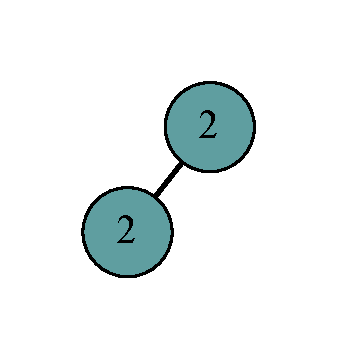
\includegraphics[scale=0.35]{Delta3TriangleFree/1[2,2].pdf}
		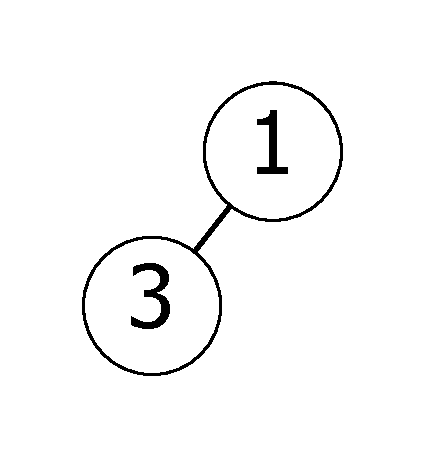
\includegraphics[scale=0.35]{Delta3TriangleFree/1[3,1].pdf}
		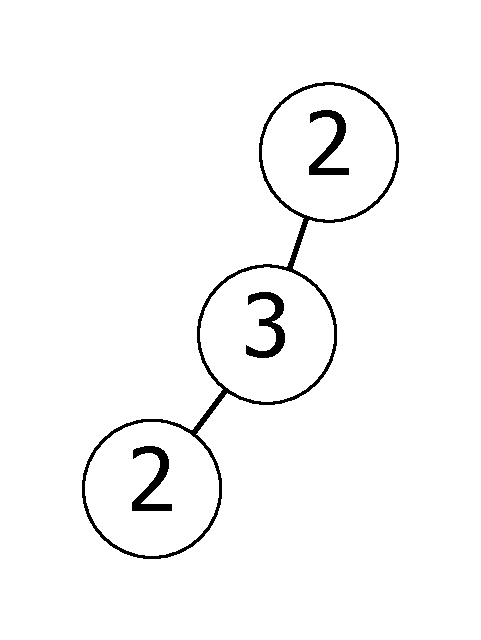
\includegraphics[scale=0.35]{Delta3TriangleFree/011[2,2,3].pdf}
		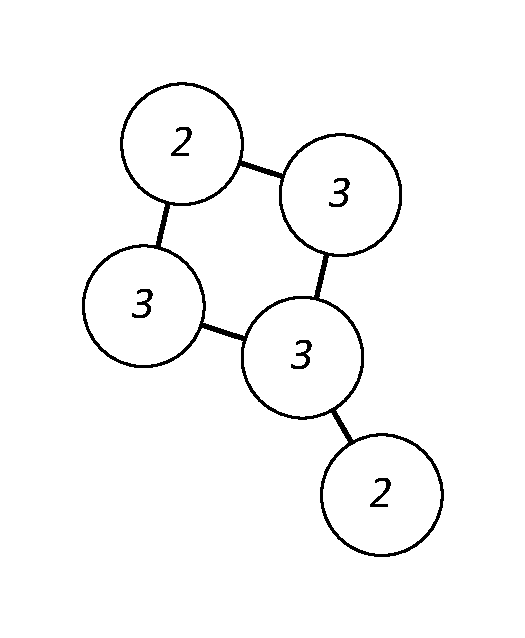
\includegraphics[scale=0.35]{Delta3TriangleFree/0011011010[3,3,2,2,3].pdf}
		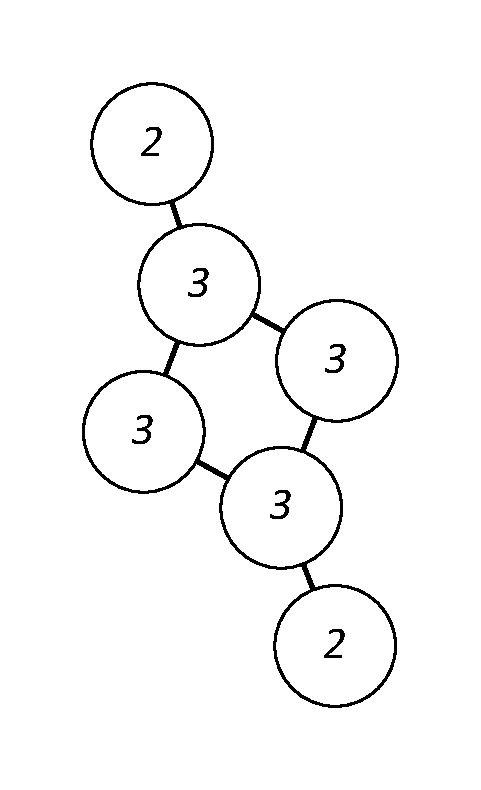
\includegraphics[scale=0.35]{Delta3TriangleFree/000110011010010[3,3,2,2,3,3].pdf}
     	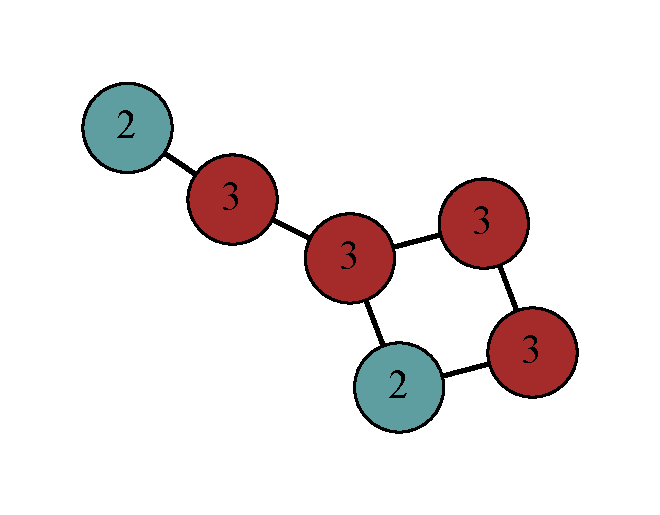
\includegraphics[scale=0.35]{Delta3TriangleFree/001010011011000[3,3,2,2,3,3].pdf}
     	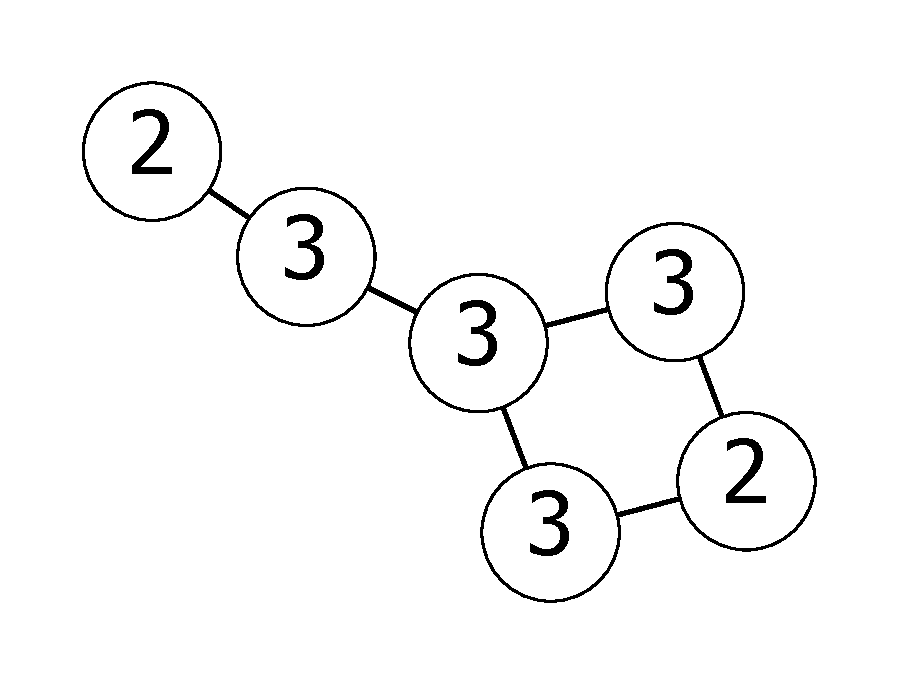
\includegraphics[scale=0.35]{Delta3TriangleFree/001010011011000[3,3,3,2,2,3].pdf}
     	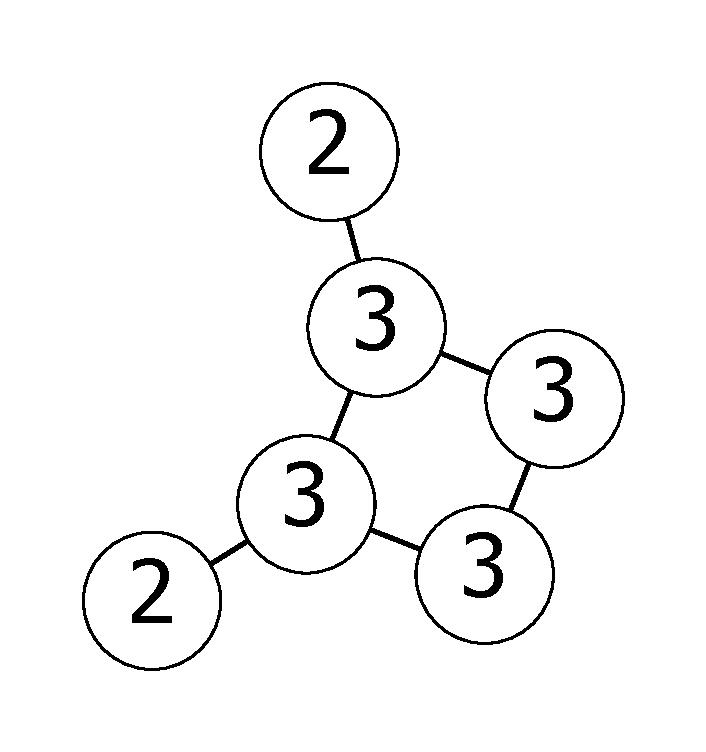
\includegraphics[scale=0.35]{Delta3TriangleFree/001110011001000[3,3,2,2,3,3].pdf}
     	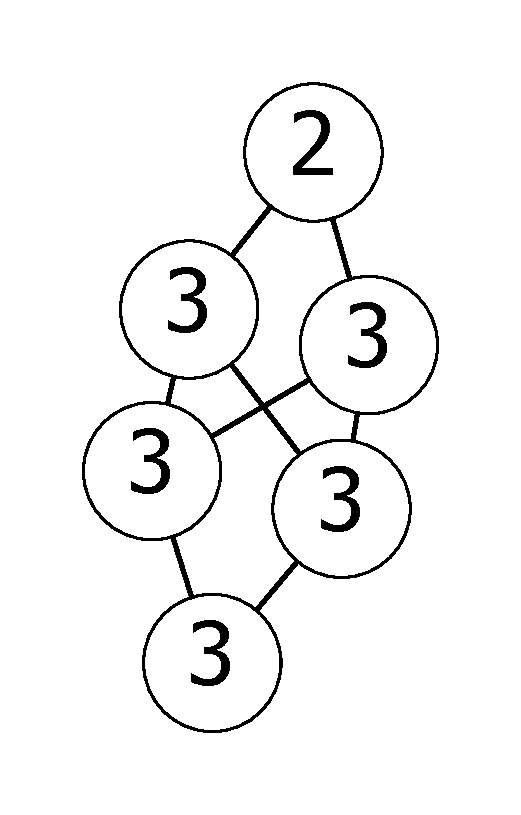
\includegraphics[scale=0.35]{Delta3TriangleFree/001110111011000[3,3,3,2,3,3].pdf}
     	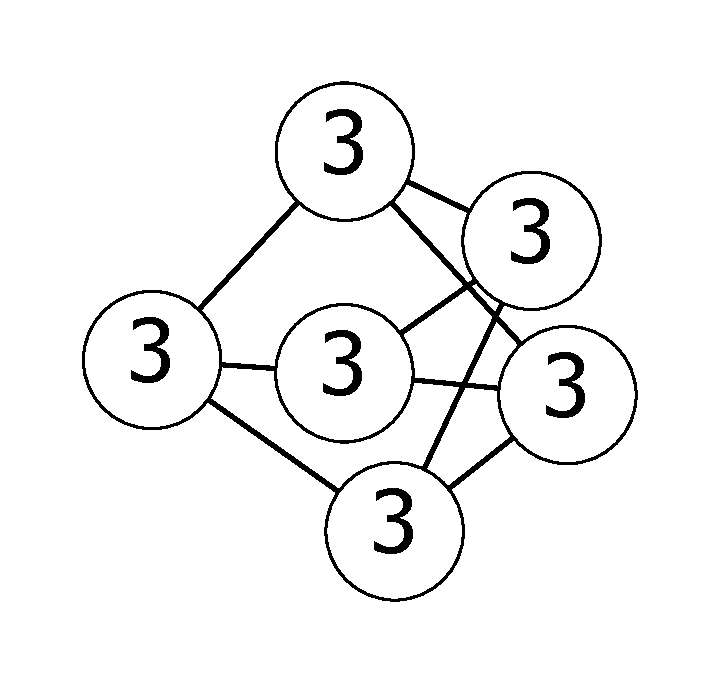
\includegraphics[scale=0.35]{Delta3TriangleFree/001110111111000[3,3,3,3,3,3].pdf}
     	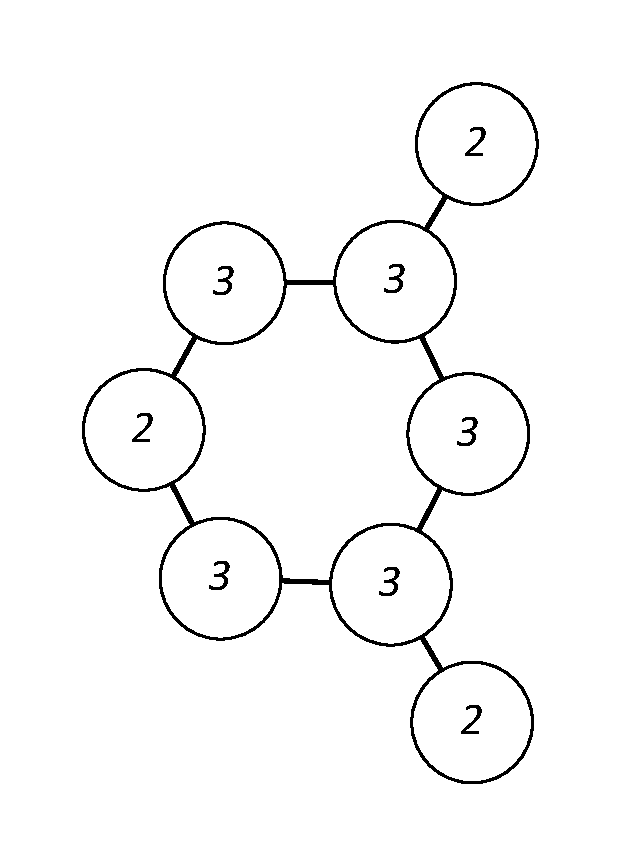
\includegraphics[scale=0.35]{Delta3TriangleFree/0000110000101000110010001000[3,3,3,2,2,2,3,3].pdf}
		\caption{Some small $3$-fixable graphs.}
		\label{fig:small3}
		\end{figure}

The penultimate graph in Figure \ref{fig:small3} is an example of the more general fact that a $k$-regular graph with $f(v) = k$ for all $v$ is $k$-fixable just is case it is $k$-edge-colorable.  That the third graph in Figure \ref{fig:small3} is reducible follows from Vizing's Adjacency Lemma.
\subsection{A necessary condition}
Since the edges incident to a given vertex must all get different colors, we have the following.

\begin{lem}\label{DegreeNecessaryCondition}
If $G$ is $(L, P)$-fixable, then $|L(v)| \ge d_G(v)$ for all $v \in V(G)$.
\end{lem}

By considering the maximum size of matchings in each color, we get a more interesting necessary condition.
For $C \subseteq \pot(L)$ and $H \subseteq G$, let $H_{L, C}$ be the
subgraph of $H$ induced on the vertices $v$ with $L(v) \cap C \ne \emptyset$. 
When $L$ is clear from context, we may write $H_C$ for $H_{L,C}$. If $C =
\set{\alpha}$, we may write $H_\alpha$ for $H_C$.  For $H \subseteq G$, put

\[\psi_L(H) = \sum_{\alpha \in \pot(L)} \floor{\frac{\card{H_{L, \alpha}}}{2}}.\]

Each term in the sum gives an upper bound on the size of a matching in color
$\alpha$. So $\psi_L(H)$ is an upper bound on the number of edges in a
partial $L$-edge-coloring of $H$.  We say that $(H, L)$ is \emph{abundant} if
$\psi_L(H) \ge \size{H}$ and that $(G,L)$ is \emph{superabundant} if for every
$H \subseteq G$, the pair $(H, L)$ is abundant.  

\begin{lem}\label{SuperabundanceIsNecessary}
If $G$ is $(L, P)$-fixable, then $(G, L)$ is superabundant.
\end{lem}
\begin{proof}
Suppose to the contrary that $G$ is $(L, P)$-fixable and there is $H \subseteq G$ such that $(H, L)$ is not abundant. We show that for all different $a,b \in P$ there is a partition $X_1, \ldots, X_t$ of $S_{a,b}$ into sets of size at most two, such that for all $J \subseteq \irange{t}$, the pair $(H,L')$ is not abundant where $L'$ is formed from $L$ by swapping $a$ and $b$ in $L(v)$ for every $v \in \bigcup_{i \in J} X_i$.  Since $G$ can never be edge-colored from a list assignment that is not superabundant, this contradicts the $(L,P)$-fixability of $G$.

Pick different $a,b \in P$.  Let $S = S_{L,a,b} \cap V(H)$ and let $S_a$ be the $v \in S$ with $a \in L(v)$.  Put $S_b = S\setminus S_a$.  Swapping $a$ and $b$ will only effect the terms $\floor{\frac{\card{S_a}}{2}}$ and $\floor{\frac{\card{S_b}}{2}}$ in $\psi_L(H)$.  So, if $\psi_L(H)$ is increased by the swapping, it must be that both $|S_a|$ and $|S_b|$ are odd and after swapping they are both even.  Say $S_a = \set{a_1, \ldots,a_p}$ and $S_b = \set{b_1, \ldots,b_q}$.  By symmetry, we may assume $p \le q$.  For $i \in \irange{p}$, let $X_i = \set{a_i, b_i}$.  Since both $p$ and $q$ are odd, $q-p$ is even, so we get a partition by, for each $j \in \irange{\frac{q-p}{2}}$, letting $X_{p + j} = \set{b_{p + 2j - 1}, b_{p + 2j}}$.  For any $i \in \irange{p}$, swapping $a$ and $b$ in $L(v)$ for every $v \in X_i$ maintains $|S_a|$ and $|S_b|$.  For any $j \in \irange{\frac{q-p}{2}}$, swapping $a$ and $b$ in $L(v)$ for every $v \in X_{p+j}$ maintains the parity of $|S_a|$ and $|S_b|$.  So no choice of $J$ can increase $\psi_L(H)$ and hence $(H,L')$ is never abundant.
\end{proof}

In particular, we have learned the following.

\begin{cor}
	If $G$ is $(f,k)$-fixable, then $(G,L)$ is superabundant for every $L$ with $L(v) \subseteq \irange{k}$ and $|L(v)| \ge k + d_{G}(v) - f(v)$ for all $v \in V(G)$.
\end{cor}

Intuitively, superabundance requires the potential for a large enough matching in each color. If instead we require the existence of a large enough matching in each color, we get a stronger condition that has been studied before. For a multigraph $H$, let $\nu(H)$ be the number of edges in a maximum matching of $H$. 
For a list assignment $L$ on $H$, put $\eta_L(H) = \sum_{\alpha \in \pot(L)} \nu(H_\alpha)$.  Note that we always have $\psi_L(H) \ge \eta_L(H)$.

The following generalization of Hall's theorem was proved by Marcotte and Seymour \cite{marcotte1990extending} and independently by Cropper, Gy{\'a}rf{\'a}s and Lehel \cite{cropper2003edge}.  By a \emph{multitree} we mean a tree that possibly has edges of multiplicity greater than one.

\begin{lem}[Marcotte and Seymour]\label{MultiTreeHall}
Let $T$ be a multitree and $L$ a list assignment on $V(T)$.  If $\eta_L(H) \ge \size{H}$ for all $H \subseteq T$, then $T$ has an $L$-edge-coloring.
\end{lem}

In \cite{HallGame}, the second author proved that superabundance is also a sufficient condition for fixability when we restrict our graphs to be multistars.  This immediately implies the fan equation.  The proof uses Hall's theorem to reduce to a smaller star and one might hope we could do the same for arbitrary trees with Lemma \ref{MultiTreeHall} in place of Hall's theorem (thus giving a short proof that Tashkinov trees are elementary), but we haven't yet been able to make this work.

\subsection{Fixability of stars}
When $G$ is a star, the conjunction of our two necessary conditions is sufficient. This generalizes Vizing fans \cite{Vizing76}; in the next section we will define ``Kierstead-Tashkinov-Vizing assignments'' and show that they are always superabundant.  In \cite{HallGame}, the second author proved a common generalization of Theorem \ref{FixabilityOfStars} and Hall's theorem, we reproduce the proof for the special case of edge-coloring.

\begin{thm}\label{FixabilityOfStars}
If $G$ is a multistar, then $G$ is weakly $L$-fixable if and only if $(G, L)$ is superabundant and $|L(v)| \ge d_G(v)$ for all $v \in V(G)$.
\end{thm}
\begin{proof}
	Our strategy is simply to increase $\eta_L(G)$ if we can; if we cannot, then Hall's theorem allows us to reduce to a smaller graph.  An easy way to describe this strategy is via a double induction as follows. Suppose the theorem is false and choose a counterexample $(G, L)$ minimizing $\size{G}$ and subject to that maximizing $\eta_L(G)$.  
	
	Let $z$ be the center of the multistar $G$. Create a bipartite graph $B$ with parts $U = \setb{zw}{E(G)}{L(z) \cap L(w) \ne \emptyset}$ and $Y \DefinedAs \setb{\alpha}{\pot(L)}{\nu(G_\alpha) = 1}$, where $zw \in U$ is adjacent to
	$\alpha \in Y$ if and only if $\alpha \in L(z) \cap L(w)$. Informally, $Y$ is
	the set of colors $\alpha$ that can be used on at least one edge, and $U$ is
	the set of edges $e$ with at least one color available on $e$, and a
	color $\alpha$ is adjacent to an edge $e$ if $\alpha$ can be used on $e$.
	
	First, suppose $|Y| < \size{G}$.  Since $|L(z)| \ge d_G(z) = \size{G}$ , we have $\tau \in L(z)$ with $\nu(G_{L, \tau}) = 0$.  Suppose there is $\beta \in Y$ such that $\card{N_B(\beta)} \ge 3$.  Pick $zw \in N_B(\beta)$.  
	Since $G$ is not $L$-fixable, there is $X \subseteq S_{L, \tau, \beta}$ with $|X| \le 2$ and $w \in X$ such that $G$ not $L'$-fixable where $L'$ is formed from $L$ by swapping $\tau$ and $\beta$ in $L(v)$ for every $v \in X$.  Since $\card{N_B(\beta)} \ge 3$, we have $\nu(G_{L', \beta}) = 1$ and $\nu(G_{L', \tau}) = 1$ and thus $\eta_{L'}(G) > \eta_L(G)$.  Since $(G,L')$ is still superabundant, this violates maximality of $\eta_L(G)$.  Hence, we must have $\card{N_B(\beta)} \le 2$ for each $\beta \in Y$.  So, each color in $Y$ contributes at most one to $\psi_L(G)$.  Since $|Y| < \size{G} \le \psi_L(G)$, there must be $\gamma \not \in Y$ such that $|G_\gamma - z| \ge 2$.  Since $G$ is not $L$-fixable, there is $X \subseteq S_{L, \tau, \gamma}$ with $|X| \le 2$ and $z \in X$ such that $G$ is not $L'$-fixable where $L'$ is formed from $L$ by swapping $\tau$ and $\gamma$ in $L(v)$ for every $v \in X$.  Since $\nu(G_{L, \tau}) = 0$ and $\nu(G_{L, \gamma}) = 0$ and $\nu(G_{L, \gamma}) = 1$, we have $\eta_{L'}(G) > \eta_L(G)$. Since $(G,L')$ is still superabundant, this violates maximality of $\eta_L(G)$.
	
	Hence we must have $|Y| \ge \size{G}$.  In particular, $\card{N_B(Y)} \le |Y|$ so we may choose $\emptyset \ne C \subseteq Y$ minimal such that $\card{N_B(C)} \le |C|$. We claim that $\card{N_B(C)} = |C|$ and there is a perfect matching $M$ of $C$ into $N_B(C)$.  Since $\card{N_B(C)} \ge 1$, this is true if $|C| = 1$.  Otherwise, for any $\tau \in C$, minimality of $C$ shows that $\card{N_B(C \setminus \set{\tau})} > |C| - 1$. Hence $\card{N_B(C)} = |C|$ and Hall's theorem gives the desired perfect matching of $C$ into $N_B(C)$.  For each $\set{zw, \alpha} \in M$, use color $\alpha$ on edge $zw$.  Form $G'$ from $G$ by removing all the colored edges and then discarding any isolated vertices. For $v \in V(G')$, let $L'(v) = L(v) \setminus C$.  Since $G$ is not $L$-fixable and $C$ and $\pot(L')$ are disjoint it must be that $G'$ is not $L'$-fixable.  Since each vertex lost exactly one color from its list for each incident edge we have $|L'(v)| \ge d_{G'}(v)$ for all $v \in V(G')$.  Also, for each $H \subseteq G'$, we have $\psi_{L'}(H) = \psi_{L}(H) - (\size{G[V(H)]} - \size{H}) \ge \size{G[V(H)]} - (\size{G[V(H)]} - \size{H}) = \size{H}$ since $H$ is abundant.  But $\size{G'} < \size{G}$, so by minimality of $\size{G}$, $G'$ is $L'$-fixable, a contradiction.
\end{proof}

\subsection{Kierstead-Tashkinov-Vizing assignments}
Many edge-coloring results have been proved using a specific kind of
superabundant pair $(G, L)$ where superabundance can be proved via a special
ordering. That is, the orderings given by the definition of Vizing fans,
Kierstead paths, and Tashkinov trees.  In this section, we show how
superabundance easily follows from these orderings.

We say that a list assignment $L$ on $G$ is a \emph{Kierstead-Tashkinov-Vizing} assignment (henceforth \emph{KTV-assignment}) if for some $xy \in E(G)$, there is a total ordering `$<$' of $V(G)$ such that

\begin{enumerate}
\item there is an edge-coloring $\pi$ of $G-xy$ such that $\pi(uv) \in L(u) \cap L(v)$ for each $uv \in E(G - xy)$; 
\item $x < z$ for all $z \in V(G - x)$; 
\item $G\brackets{w \mid w \le z}$ is connected for all $z \in V(G)$; 
\item for each $wz \in E(G - xy)$, there is $u < \max\set{w, z}$ such that $\pi(wz) \in L(u) - \setbs{\pi(e)}{e \in E(u)}$;
\item there are different $s, t \in V(G)$ such that $L(s) \cap L(t) - \setbs{\pi(e)}{e \in E(s) \cup E(t)} \ne \emptyset$.
\end{enumerate}

\begin{lem}\label{KTVImpliesSuperabundant}
If $L$ is a KTV-assignment on $G$, then $(G, L)$ is superabundant.
\end{lem}
\begin{proof}
Let $L$ be a KTV-assignment on $G$, and let $H \subseteq G$.  We will show that
$(H,L)$ is abundant.  
Clearly it suffices to consider the case when $H$ is an induced subgraph, so we
assume this.
Property (1) gives that $G-xy$ has an edge-coloring
$\pi$, so $\psi_L(H)\ge \size{H}-1$; also $\psi_L(H)\ge \size{H}$ if
$\{x,y\}\not\subseteq V(H)$.  Furthermore $\psi_L(H)\ge \size{H}$ if $s$ and
$t$ from property (5) are both in $V(H)$, since then $\psi_L(H)$ gains 1 over
the naive lower bound, due to the color in $L(s)\cap L(t)$.  So $V(G)-
V(H)\ne \emptyset$.

Now choose $z \in V(G) - V(H)$ that is smallest under $<$.  
Put $H' = G\brackets{w \mid w \le z}$.  By the minimality of $z$, we have $H' - z \subseteq H$. By property (2), $\card{H'} \ge 2$.  
By property (3), $H'$ is connected and thus there is $w \in V(H' - z)$ adjacent to $z$. So, we have $w < z$ and $wz\in E(G)-E(H)$.
Now $\pi(wz)\in L(w)$.  By the definition of a KTV-assignment, 
property (4) implies that there exists $u$ with $u < \max\set{w, z} = z$ and $\pi(wz) \in
L(u)-\{\pi(e)|e\in E(u)\}$.  Then $u \in V(H' - z) \subseteq V(H)$ and
again we gain 1 over the naive lower bound on $\psi_L(H)$, due to the color
in $L(u)\cap L(w)$.  So $\psi_L(H)\ge \size{H}$.
\end{proof}

\section{Applications of small k-fixable graphs}
\subsection{Impoved lower bound on the average degree of 3-critical graphs}
\subsection{Impoved lower bound on the average degree of 4-critical graphs}
\subsection{The conjecture of Hilton and Zhao for $\Delta=4$}
For a graph $G$, let $G_\Delta$ be the subgraph of $G$ induced on vertices of degree $\Delta(G)$.  Vizing's Adjacency Lemma implies that $\delta(G_\Delta) \ge 2$ in a critical graph $G$.  A natural question is whether or not this is the best we can do.  For example, is it possible that $\Delta(G_\Delta) = 2$ in a critical graph $G$?  It turns out that it is and a conjecture of Hilton and Zhao says when exactly this can happen.  A graph $G$ is \emph{overfull} if $||G|| > \floor{\frac{|G|}{2}}\Delta(G)$.  Let $P^*$ be the Peterson graph with one vertex removed (ADD PICTURE).

\begin{conjecture}[Hilton and Zhao]
A connected graph $G$ with $\Delta(G_\Delta) \le 2$ is class 2 if and only if $G$ is $P^*$ or $G$ is overfull.
\end{conjecture}

David and Gianfranco Cariolaro proved this conjecture for the $\Delta=3$ case \cite{cariolaro2003colouring}.  Here we prove the $\Delta=4$ case, but do not include the very long computer generated proofs of the reducibility of the graphs in Figure~\ref{fig:hiltonzhao}.  Not all of the graphs in Figure~\ref{fig:hiltonzhao} are $4$-fixable; to prove reducibility of a graph $H$, we restrict the allowed list assignments on vertices to those from which all but one edge of $H$ can be colored.  Such a list assignment is called a \emph{nearly-colorable}.  Checking only the nearly-colorable assignments clearly suffices for reducibility.


\begin{figure}
	\centering
	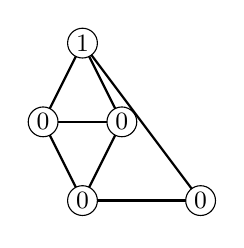
\begin{tikzpicture}[scale = 5]
	\tikzstyle{VertexStyle} = []
	\tikzstyle{EdgeStyle} = []
	\tikzstyle{labeledStyle}=[shape = circle, minimum size = 6pt, inner sep = 1.2pt, draw]
	\tikzstyle{unlabeledStyle}=[shape = circle, minimum size = 6pt, inner sep = 1.2pt, draw, fill]
	\Vertex[style = labeledStyle, x = 0.550, y = 0.650, L = \small {$1$}]{v0}
	\Vertex[style = labeledStyle, x = 0.550, y = 0.250, L = \small {$0$}]{v1}
	\Vertex[style = labeledStyle, x = 0.450, y = 0.450, L = \small {$0$}]{v2}
	\Vertex[style = labeledStyle, x = 0.850, y = 0.250, L = \small {$0$}]{v3}
	\Vertex[style = labeledStyle, x = 0.650, y = 0.450, L = \small {$0$}]{v4}
	\Edge[label = \small {}, labelstyle={auto=right, fill=none}](v0)(v2)
	\Edge[label = \small {}, labelstyle={auto=right, fill=none}](v0)(v3)
	\Edge[label = \small {}, labelstyle={auto=right, fill=none}](v0)(v4)
	\Edge[label = \small {}, labelstyle={auto=right, fill=none}](v1)(v2)
	\Edge[label = \small {}, labelstyle={auto=right, fill=none}](v1)(v3)
	\Edge[label = \small {}, labelstyle={auto=right, fill=none}](v1)(v4)
	\Edge[label = \small {}, labelstyle={auto=right, fill=none}](v2)(v4)
	\end{tikzpicture}
	\label{fig:SubdividedK4}
	\centering
	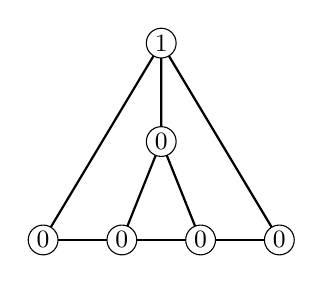
\begin{tikzpicture}[scale = 5]
	\tikzstyle{VertexStyle} = []
	\tikzstyle{EdgeStyle} = []
	\tikzstyle{labeledStyle}=[shape = circle, minimum size = 6pt, inner sep = 1.2pt, draw]
	\tikzstyle{unlabeledStyle}=[shape = circle, minimum size = 6pt, inner sep = 1.2pt, draw, fill]
	\Vertex[style = labeledStyle, x = 0.650, y = 0.300, L = \small {$0$}]{v0}
	\Vertex[style = labeledStyle, x = 0.550, y = 0.800, L = \small {$1$}]{v1}
	\Vertex[style = labeledStyle, x = 0.450, y = 0.300, L = \small {$0$}]{v2}
	\Vertex[style = labeledStyle, x = 0.850, y = 0.300, L = \small {$0$}]{v3}
	\Vertex[style = labeledStyle, x = 0.250, y = 0.300, L = \small {$0$}]{v4}
	\Vertex[style = labeledStyle, x = 0.550, y = 0.550, L = \small {$0$}]{v5}
	\Edge[label = \small {}, labelstyle={auto=right, fill=none}](v0)(v2)
	\Edge[label = \small {}, labelstyle={auto=right, fill=none}](v0)(v3)
	\Edge[label = \small {}, labelstyle={auto=right, fill=none}](v0)(v5)
	\Edge[label = \small {}, labelstyle={auto=right, fill=none}](v1)(v3)
	\Edge[label = \small {}, labelstyle={auto=right, fill=none}](v1)(v4)
	\Edge[label = \small {}, labelstyle={auto=right, fill=none}](v1)(v5)
	\Edge[label = \small {}, labelstyle={auto=right, fill=none}](v2)(v4)
	\Edge[label = \small {}, labelstyle={auto=right, fill=none}](v2)(v5)
	\end{tikzpicture}
	\caption{These are AT.}
	\label{fig:TriangleRuinsPath}
\end{figure}

\begin{figure}
	\centering
	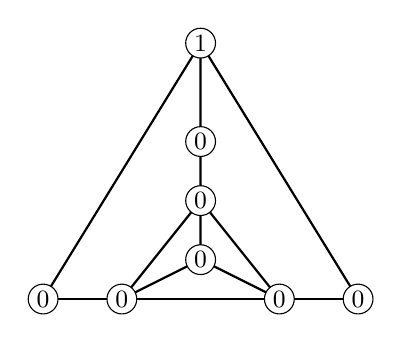
\begin{tikzpicture}[scale = 5]
	\tikzstyle{VertexStyle} = []
	\tikzstyle{EdgeStyle} = []
	\tikzstyle{labeledStyle}=[shape = circle, minimum size = 6pt, inner sep = 1.2pt, draw]
	\tikzstyle{unlabeledStyle}=[shape = circle, minimum size = 6pt, inner sep = 1.2pt, draw, fill]
	\Vertex[style = labeledStyle, x = 0.850, y = 0.300, L = \small {$0$}]{v0}
	\Vertex[style = labeledStyle, x = 0.850, y = 0.600, L = \small {$0$}]{v1}
	\Vertex[style = labeledStyle, x = 1.250, y = 0.200, L = \small {$0$}]{v2}
	\Vertex[style = labeledStyle, x = 0.450, y = 0.200, L = \small {$0$}]{v3}
	\Vertex[style = labeledStyle, x = 0.850, y = 0.450, L = \small {$0$}]{v4}
	\Vertex[style = labeledStyle, x = 1.050, y = 0.200, L = \small {$0$}]{v5}
	\Vertex[style = labeledStyle, x = 0.850, y = 0.850, L = \small {$1$}]{v6}
	\Vertex[style = labeledStyle, x = 0.650, y = 0.200, L = \small {$0$}]{v7}
	\Edge[label = \small {}, labelstyle={auto=right, fill=none}](v0)(v4)
	\Edge[label = \small {}, labelstyle={auto=right, fill=none}](v0)(v5)
	\Edge[label = \small {}, labelstyle={auto=right, fill=none}](v0)(v7)
	\Edge[label = \small {}, labelstyle={auto=right, fill=none}](v1)(v4)
	\Edge[label = \small {}, labelstyle={auto=right, fill=none}](v1)(v6)
	\Edge[label = \small {}, labelstyle={auto=right, fill=none}](v2)(v5)
	\Edge[label = \small {}, labelstyle={auto=right, fill=none}](v2)(v6)
	\Edge[label = \small {}, labelstyle={auto=right, fill=none}](v3)(v6)
	\Edge[label = \small {}, labelstyle={auto=right, fill=none}](v3)(v7)
	\Edge[label = \small {}, labelstyle={auto=right, fill=none}](v4)(v5)
	\Edge[label = \small {}, labelstyle={auto=right, fill=none}](v4)(v7)
	\Edge[label = \small {}, labelstyle={auto=right, fill=none}](v5)(v7)
	\end{tikzpicture}
%		\caption{This is AT.}
		\label{fig:thebigone}
%\end{figure}
%\begin{figure}
	\centering
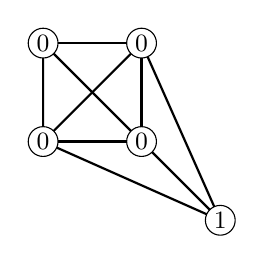
\begin{tikzpicture}[scale = 5]
\tikzstyle{VertexStyle} = []
\tikzstyle{EdgeStyle} = []
\tikzstyle{labeledStyle}=[shape = circle, minimum size = 6pt, inner sep = 1.2pt, draw]
\tikzstyle{unlabeledStyle}=[shape = circle, minimum size = 6pt, inner sep = 1.2pt, draw, fill]
\Vertex[style = labeledStyle, x = 0.550, y = 0.700, L = \small {$0$}]{v0}
\Vertex[style = labeledStyle, x = 0.550, y = 0.450, L = \small {$0$}]{v1}
\Vertex[style = labeledStyle, x = 0.800, y = 0.700, L = \small {$0$}]{v2}
\Vertex[style = labeledStyle, x = 1.000, y = 0.250, L = \small {$1$}]{v3}
\Vertex[style = labeledStyle, x = 0.800, y = 0.450, L = \small {$0$}]{v4}
\Edge[label = \small {}, labelstyle={auto=right, fill=none}](v0)(v2)
\Edge[label = \small {}, labelstyle={auto=right, fill=none}](v0)(v4)
\Edge[label = \small {}, labelstyle={auto=right, fill=none}](v1)(v0)
\Edge[label = \small {}, labelstyle={auto=right, fill=none}](v1)(v3)
\Edge[label = \small {}, labelstyle={auto=right, fill=none}](v1)(v4)
\Edge[label = \small {}, labelstyle={auto=right, fill=none}](v2)(v1)
\Edge[label = \small {}, labelstyle={auto=right, fill=none}](v2)(v4)
\Edge[label = \small {}, labelstyle={auto=right, fill=none}](v3)(v2)
\Edge[label = \small {}, labelstyle={auto=right, fill=none}](v4)(v3)
\end{tikzpicture}
	\caption{These are AT.}
	\label{fig:K5minus}
\end{figure}

Since we do not include the reducibility proofs, we separate the proof into two parts.  The first does not use the computer at all.
Let $\H_4$ be the class of connected graphs with maximum degree 4, minimum
degree 3, each vertex adjacent to at least two 4-vertices, and each 4-vertex
adjacent to exactly two 4-vertices.
\begin{lem}\label{HiltonZhaoLemma}
	If $G$ is a graph in $\H_4$ and $G$ contains none of the four configurations in Figure~\ref{fig:hiltonzhao}
	(not necessarily induced), then $G$ is $K_5-e$.
\end{lem}
\begin{proof}
	Let $G$ be a graph in $\H_4$.  Note that every 4-vertex in $G$ has exactly two
	3-neighbors and two 4-neighbors.
	Let $u$ denote a 4-vertex and let $v_1,\ldots,v_4$ denote its neighbors, where
	$d(v_1)=d(v_2)=3$ and $d(v_3)=d(v_4)=4$.
	When vertices $x$ and $y$ are adjacent, we write $x\adj y$.
	We assume that $G$ contains none of the configurations in Figure~\ref{fig:hiltonzhao} and show that
	$G$ must be $K_5-e$.  
	
	First suppose that $u$ has a 3-neighbor and a 4-neighbor that are adjacent.  By
	symmetry, suppose that $v_2$ is adjacent to $v_3$.  Since Figure~\ref{fig:hiltonzhao}(a) is forbidden,
	we have $v_3\adj v_1$. 
	Now consider $v_4$.  If $v_4$ has a 3-neighbor distinct from $v_1$ and $v_2$,
	then we have a copy of Figure~\ref{fig:hiltonzhao}(d).  Hence $v_4\adj v_1$ and $v_4\adj v_2$.
	If $v_3\adj v_4$, then $G$ is $K_5-e$.  Suppose not, and let $x$ be a 4-neighbor
	of $v_4$.  Since $G$ has no copy of Figure~\ref{fig:hiltonzhao}(d), $x$ must be adjacent to $v_1$ and
	$v_2$.  This is a contradiction, since now $v_1$ and $v_2$ are 3-vertices, but
	each have at least four neighbors.  Hence, we conclude that each of $v_1$ and
	$v_2$ is non-adjacent to each of $v_3$ and $v_4$.
	
	Now consider the 3-neighbors of $v_3$ and $v_4$.  
	If they have zero 3-neighbors in common, then we have a copy of Figure~\ref{fig:hiltonzhao}(b).  
	If they have one 3-neighbor in common, then we have a copy of Figure~\ref{fig:hiltonzhao}(c).
	Otherwise they have two 3-neighbors in common, so we have a copy of Figure~\ref{fig:hiltonzhao}(d).  
\end{proof}

Since $K_5 - e$ is overfull, the following implies Hilton and Zhao's conjecture for $\Delta=4$.
\begin{thm}
A connected graph $G$ with $\Delta(G) = 4$ and $\Delta(G_\Delta) \le 2$ is class 2 if and only if $G$ is $K_5-e$.
\end{thm}
\begin{proof}
Suppose not and choose a counterexample $G$ minimizing $\size{G}$.  If $\chi'(G-xy) = 5$ for some $xy \in E(G)$, then by minimality of $\size{G}$ some component of $G-xy$ is $K_5-e$.  But this is impossible since then one of $x$ or $y$ has at least three $4$-neighbors.  Hence $G$ is critical. By computer, the graphs in Figure~\ref{fig:hiltonzhao} are reducible and thus $G$ satisfies the hypotheses of Lemma \ref{HiltonZhaoLemma}.  Therefore, $G$ is $K_5-e$, a contradiction.
\end{proof}


\section{Superabundance sufficiency and adjacency lemmas}
	\begin{figure}[htb]
		\centering
		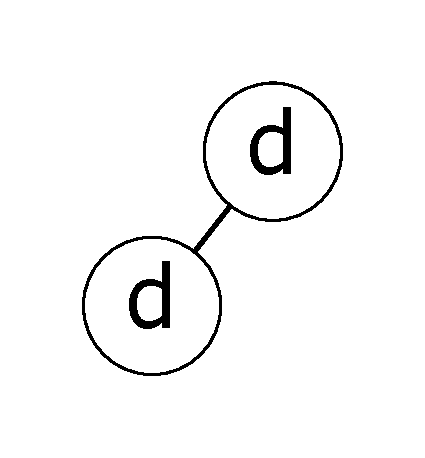
\includegraphics[scale=0.5]{Superabundance/all/1[1,1].pdf}
		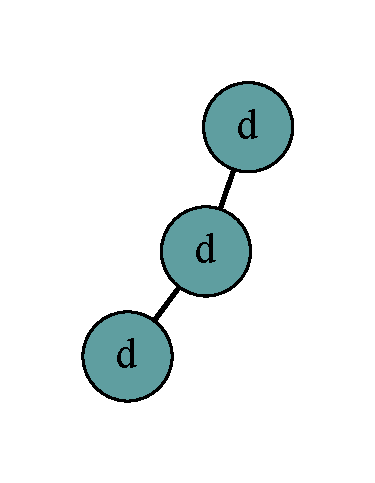
\includegraphics[scale=0.5]{Superabundance/all/011[1,1,2].pdf}
		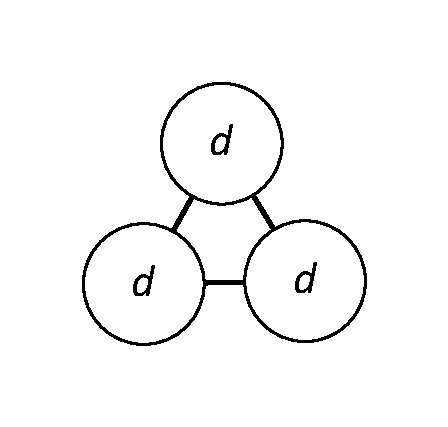
\includegraphics[scale=0.5]{Superabundance/all/111[2,2,2].pdf}
		\caption{The fixable graphs on at most 3 vertices.}
		\label{fig:fixable3}
	\end{figure}
	
	\begin{defn}
		If $G$ is a graph and $\func{f}{V(G)}{\IN}$ with $f(v) \ge d_G(v)$ for all $v \in V(G)$, then $G$ is $f$-fixable if $G$ is $(L, P)$-fixable for every $L$ with $|L(v)| \ge f(v)$ for all $v \in V(G)$ and every $L$-pot $P$ such that $(G,L)$ is superabundant.
	\end{defn}
	
	Since $f(v) \ge d_G(v)$, it is convenient to express the values of $f$ as $d+k$ for a non-negative integer $k$; this means $f(v) = d_G(v) + k$.  When $k=0$, we just write $d$ as in Figure \ref{fig:fixable3}.  
	
		\begin{figure}[htb]
					\centering
			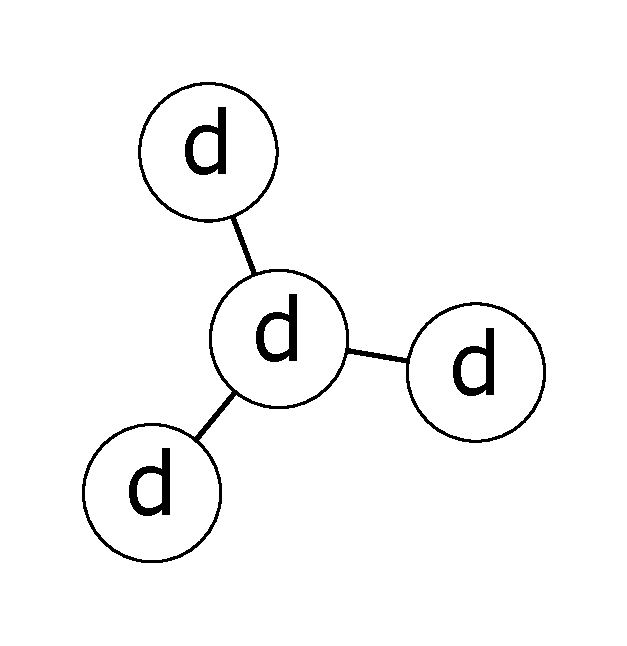
\includegraphics[scale=0.5]{Superabundance/all/001011[1,1,1,3].pdf}
			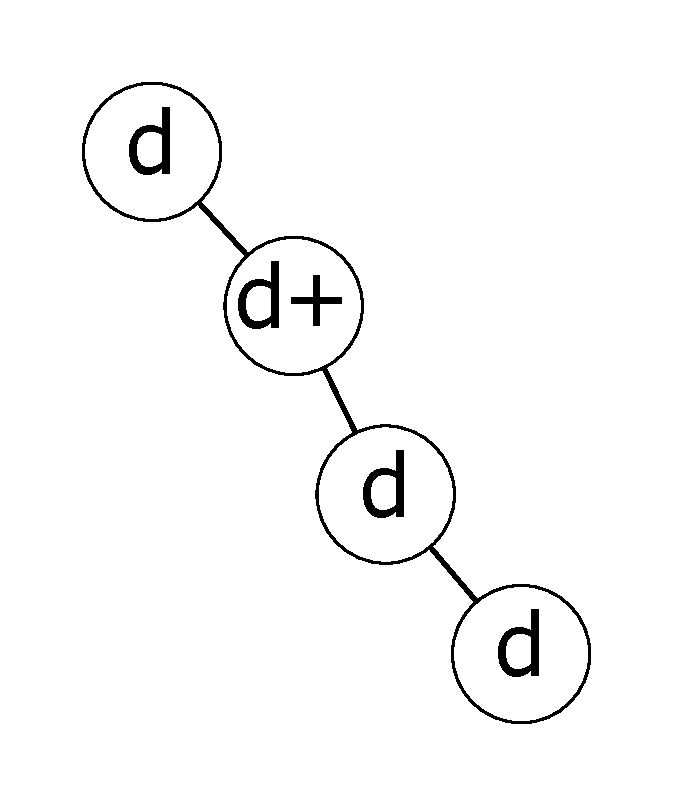
\includegraphics[scale=0.5]{Superabundance/all/011010[2,1,1,3].pdf}
			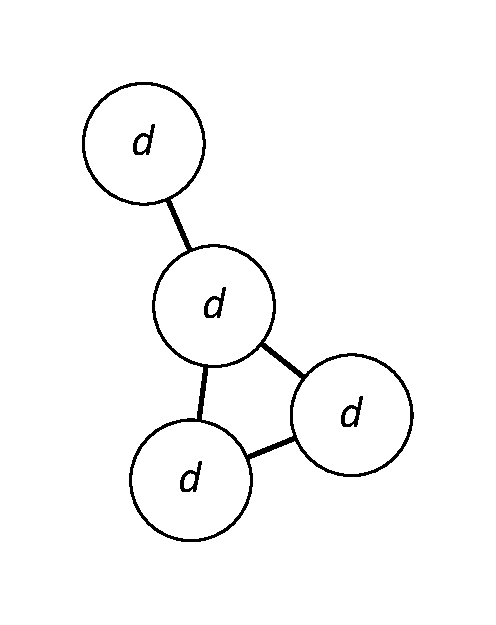
\includegraphics[scale=0.5]{Superabundance/all/011011[2,1,2,3].pdf}
			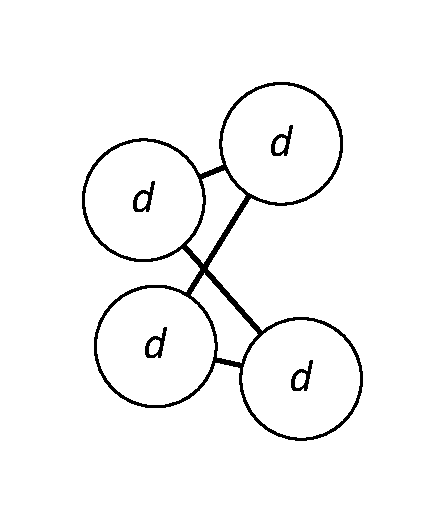
\includegraphics[scale=0.5]{Superabundance/all/011110[2,2,2,2].pdf}
			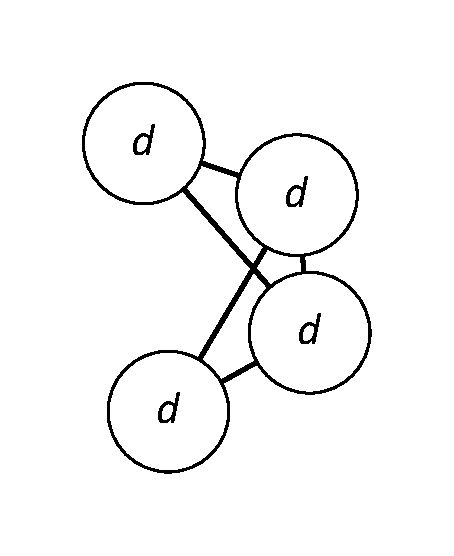
\includegraphics[scale=0.5]{Superabundance/all/011111[2,2,3,3].pdf}
			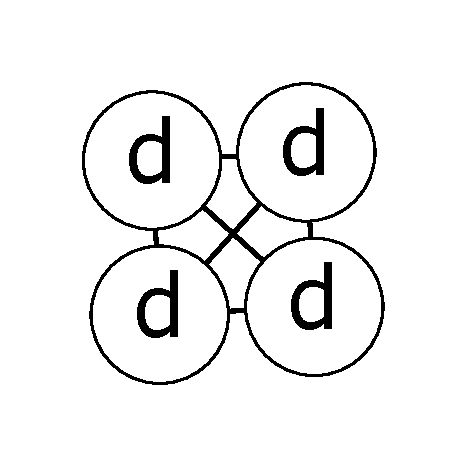
\includegraphics[scale=0.5]{Superabundance/all/111111[3,3,3,3].pdf}
			\caption{The fixable graphs on 4 vertices.}
			\label{fig:fixable4}
		\end{figure}

		
		\begin{figure}[htb]
					\centering
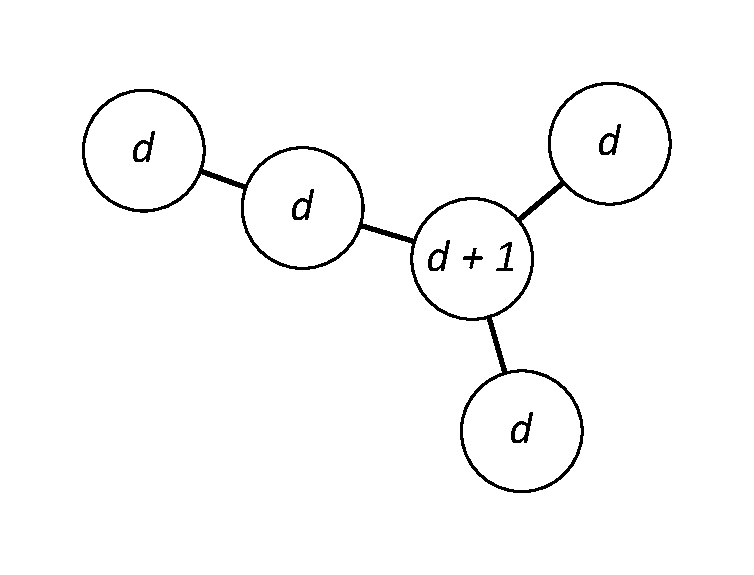
\includegraphics[scale=0.4]{Superabundance/MaxDegree3Trees/0011001010[2,1,1,1,4].pdf}
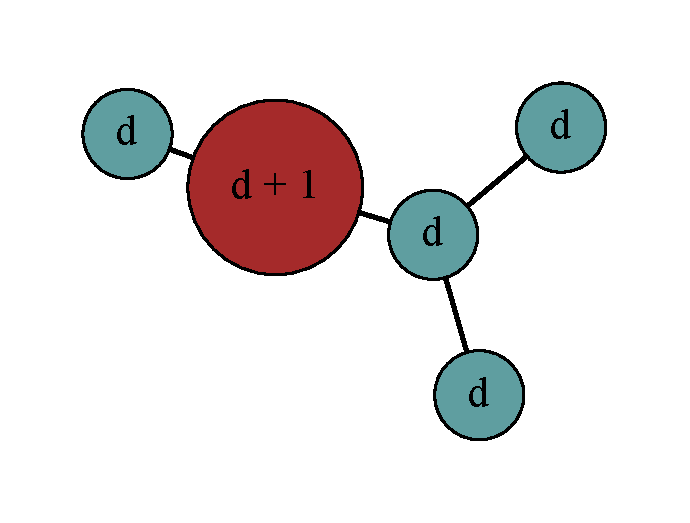
\includegraphics[scale=0.4]{Superabundance/MaxDegree3Trees/0011001010[3,1,1,1,3].pdf}
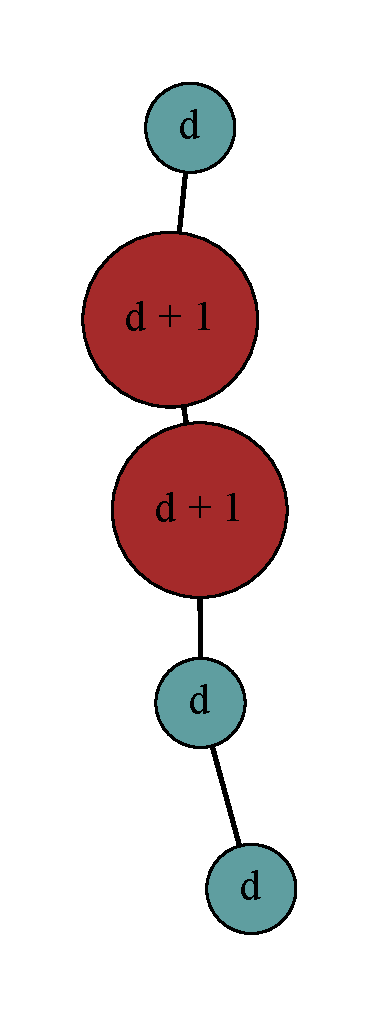
\includegraphics[scale=0.4]{Superabundance/MaxDegree3Trees/0101011000[2,3,1,1,3].pdf}
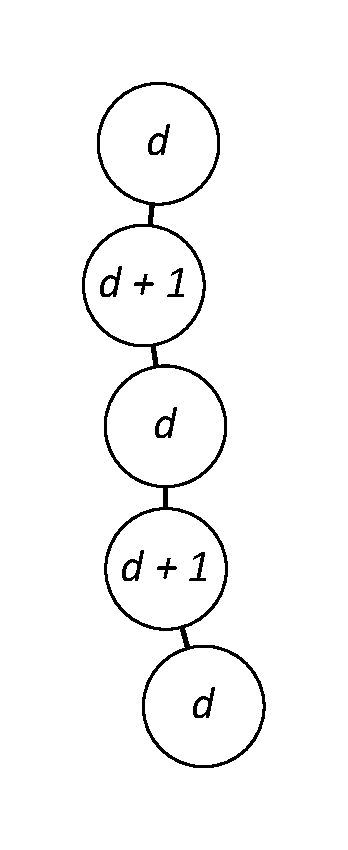
\includegraphics[scale=0.4]{Superabundance/MaxDegree3Trees/0101011000[3,3,1,1,2].pdf}
			\caption{The fixable trees with maximum degree at most 3 on 5 vertices.}
			\label{fig:fixable5tree}
		\end{figure}
		
				\begin{figure}[htb]
					\centering
					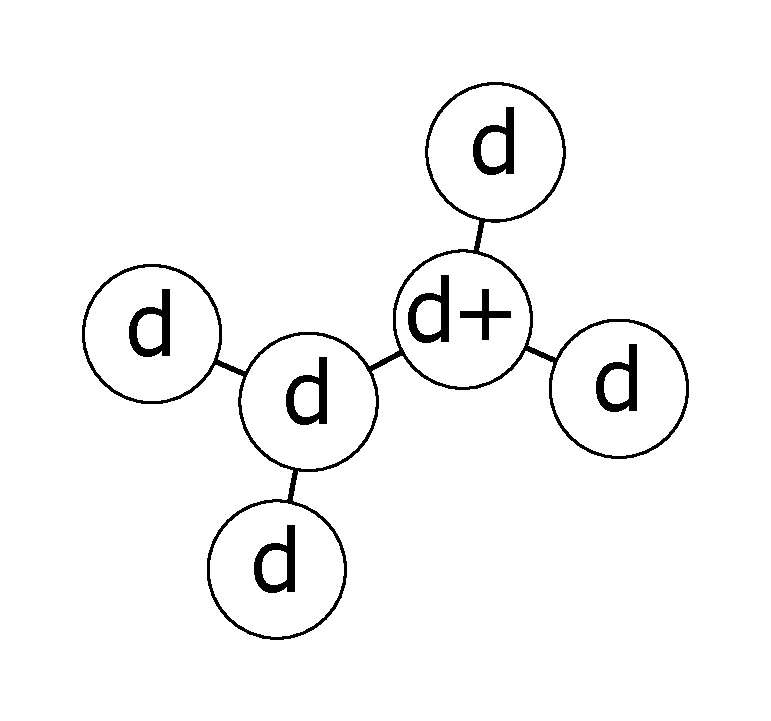
\includegraphics[scale=0.25]{Superabundance/MaxDegree3Trees/000100010001011[1,1,1,1,3,4].pdf}
					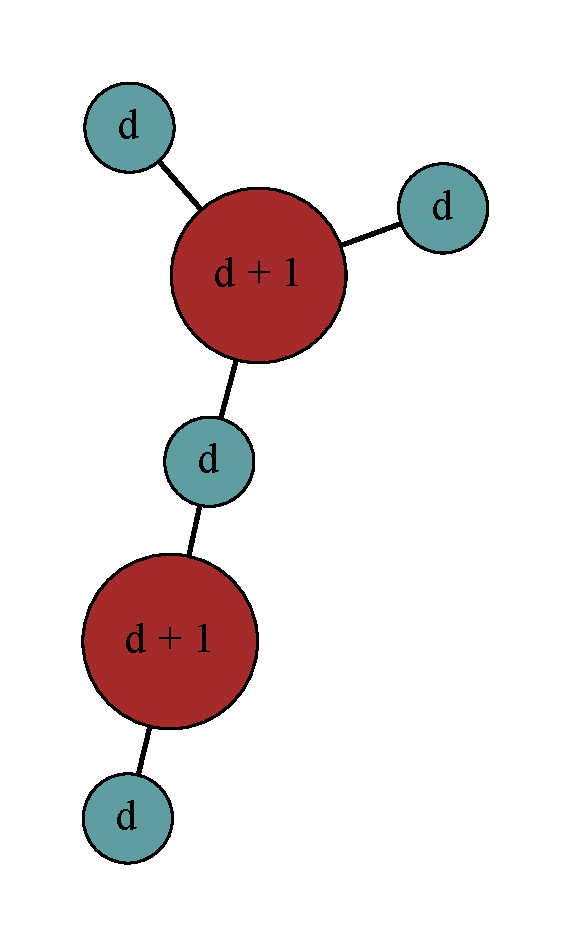
\includegraphics[scale=0.25]{Superabundance/MaxDegree3Trees/000110010001010[2,1,1,1,3,4].pdf}
					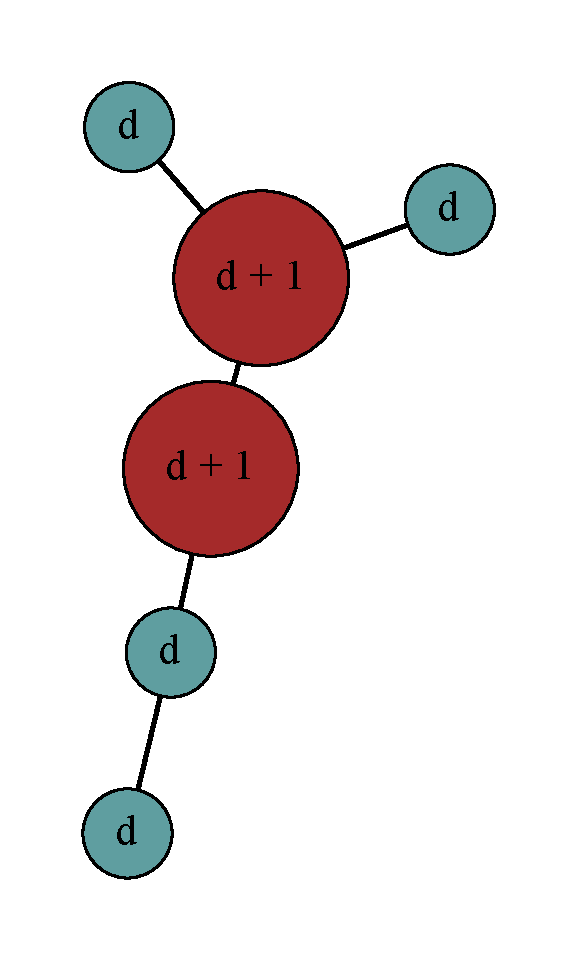
\includegraphics[scale=0.25]{Superabundance/MaxDegree3Trees/000110010001010[3,1,1,1,2,4].pdf}
					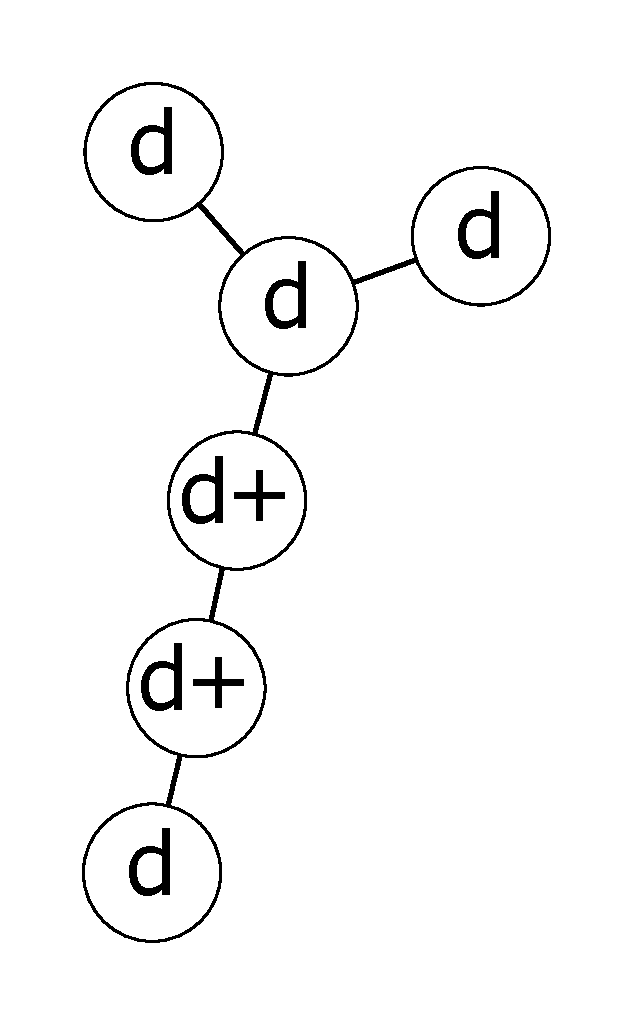
\includegraphics[scale=0.25]{Superabundance/MaxDegree3Trees/000110010001010[3,1,1,1,3,3].pdf}
					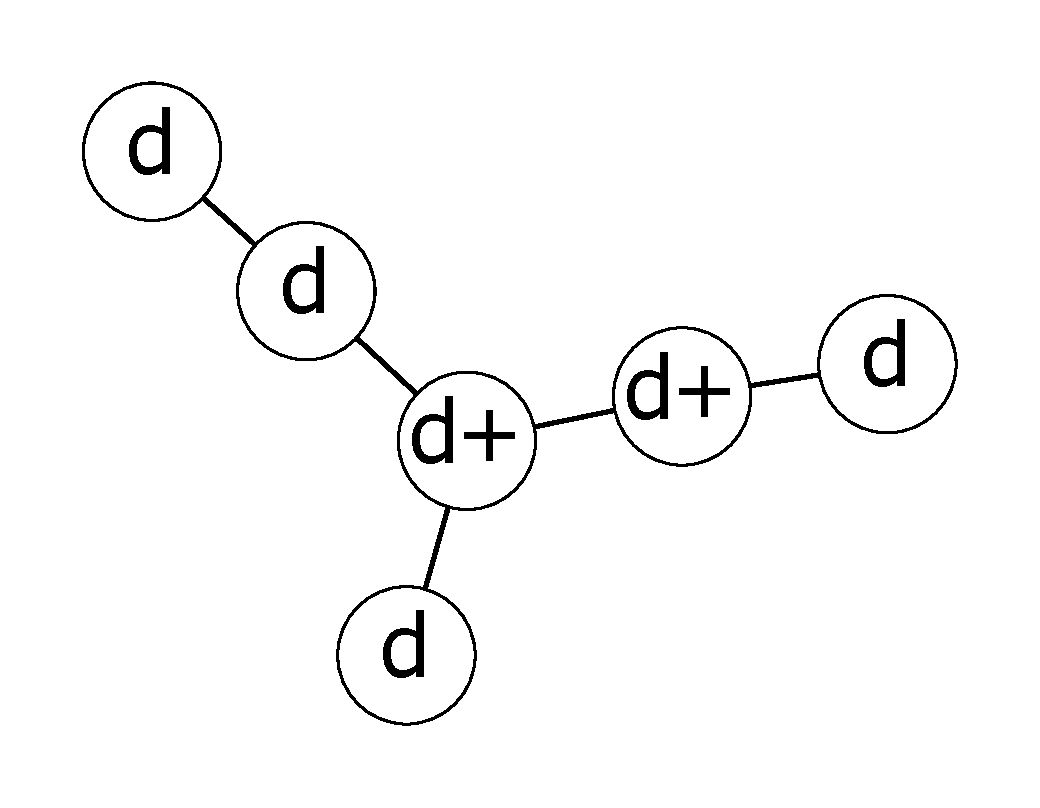
\includegraphics[scale=0.25]{Superabundance/MaxDegree3Trees/001010011001000[2,3,1,1,1,4].pdf}
					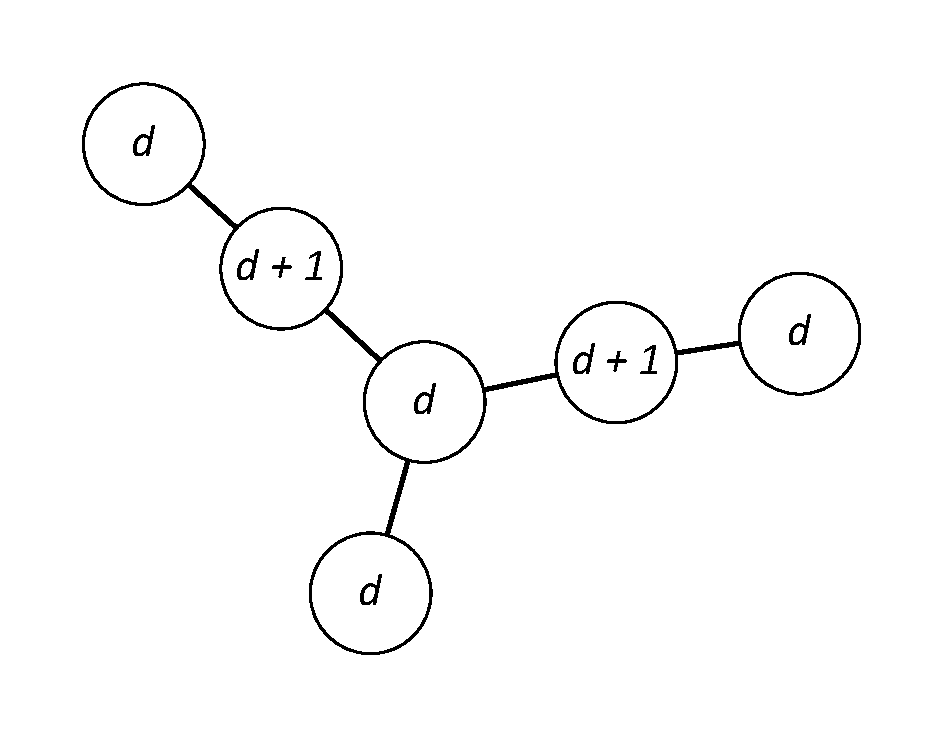
\includegraphics[scale=0.25]{Superabundance/MaxDegree3Trees/001010011001000[3,3,1,1,1,3].pdf}
					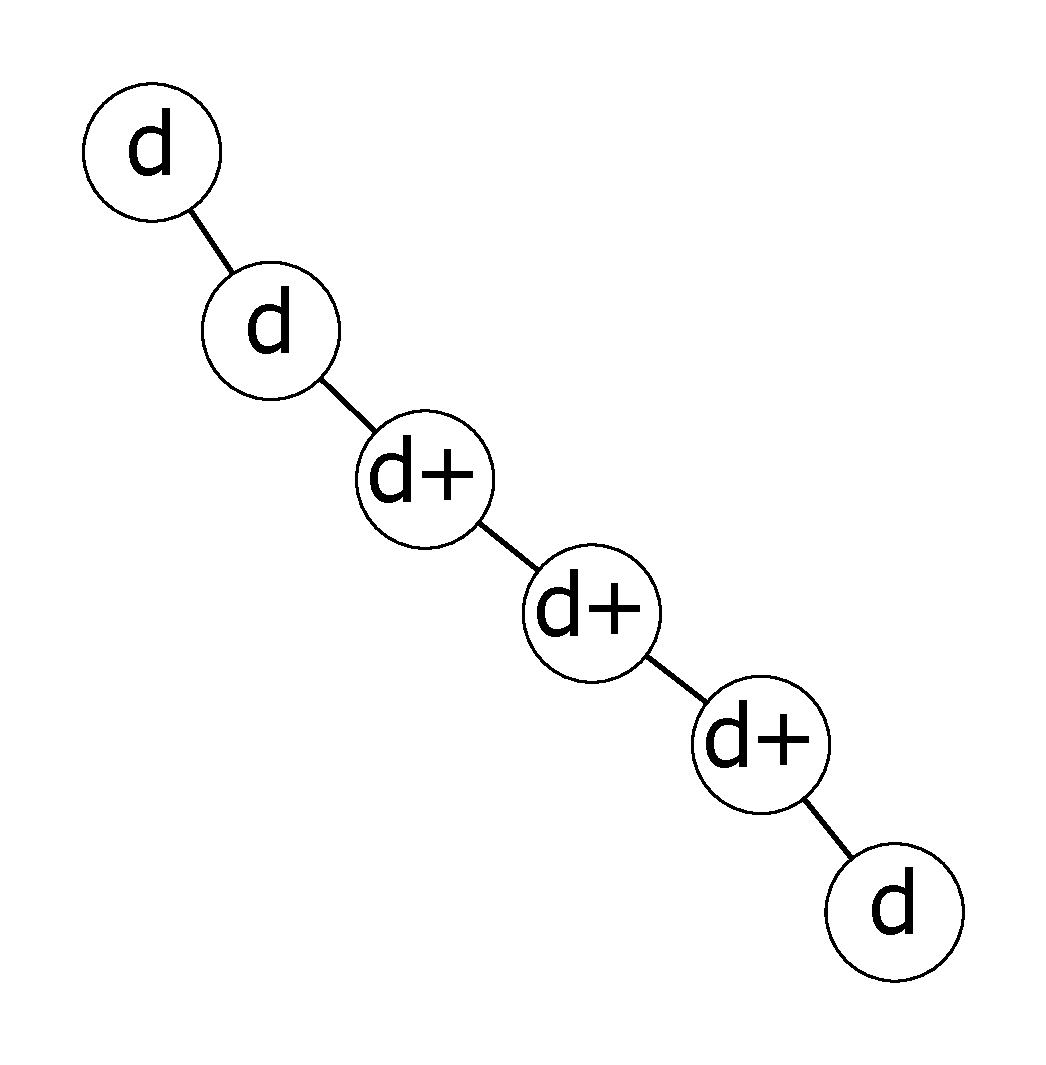
\includegraphics[scale=0.25]{Superabundance/MaxDegree3Trees/001010011010000[2,3,1,1,3,3].pdf}
					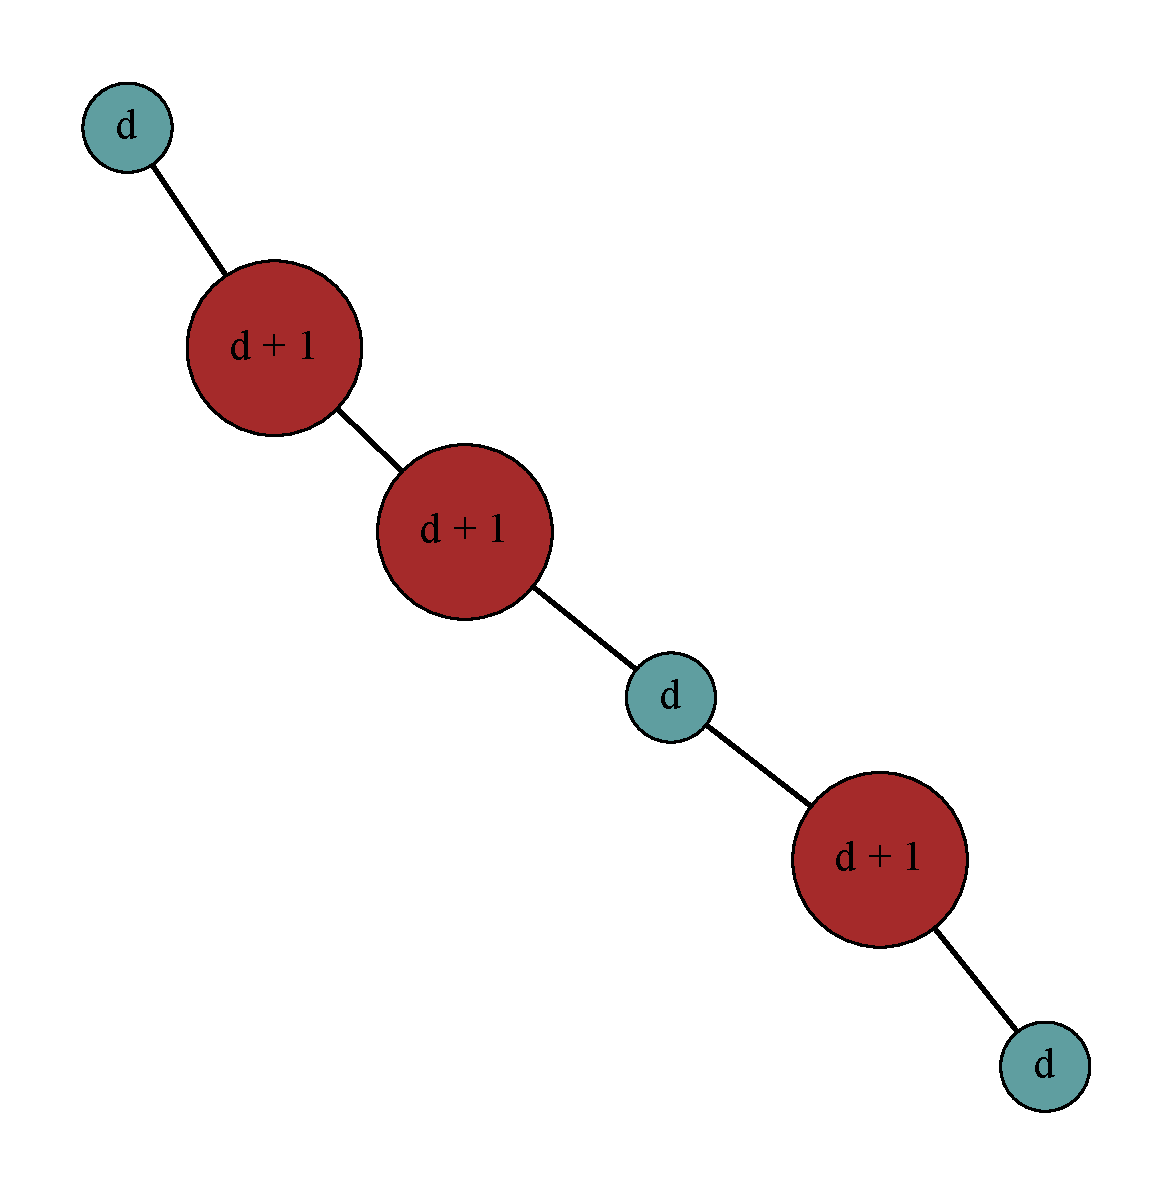
\includegraphics[scale=0.25]{Superabundance/MaxDegree3Trees/001010011010000[3,2,1,1,3,3].pdf}
					\caption{The fixable trees with maximum degree at most 3 on 6 vertices.}
					\label{fig:fixable6tree}
				\end{figure}

Looking at the trees in Figures \ref{fig:fixable4}, \ref{fig:fixable5tree} and \ref{fig:fixable6tree} we might conjecture that a tree is $f$-fixable as long as there is at most one internal vertex labeled ``d''.  This conjecture continues to hold for many more examples.

\begin{conjecture}\label{OneHighConjecture}
	A tree $T$ is $f$-fixable if $f(v) = d_T(v)$ for at most one non-leaf $v$ of $T$.
\end{conjecture}

Note that by Lemma \ref{KTVImpliesSuperabundant}, this would imply that Tashkinov trees are elementary under the same degree constraints.  Can this be proved in the simpler case of Kierstead paths?  For paths of length 4, this was done by Kostochka and Stiebitz, in the next section we present a generalization of this result to stars with one edge subdivided.   One nice feature of the superabundance formulation is that since there is no need for an ordering like with Tashkinov trees, we can easily formulate results about graphs with cycles.  The most general thing we might think is true is the following.

\begin{conjecture}[false]\label{MoonshineConjecture}
	A multigraph $G$ is $f$-fixable if $f(v) > d_G(v)$ for all $v \in V(T)$.
\end{conjecture}

This is very strong and implies Goldberg's conjecture.  Unfortunately, it is false, we can make a counterexample on a $5$-cycle. [SHOW HOW.  No change like $f(v) > d_G(v) + 100$ will help.] 
	
\subsection{Stars with one edge subdivided}
The following generalizes the ``Short Kierstead Paths'' of Kostochka and Stiebitz.  Parts (a) and (b) are a special case of Conjecture \ref{OneHighConjecture}. At present, we feel the proof we have is too involved and ugly to present, but it will be instructive to see how we can extract a fan-equation-like formula from Theorem \ref{StarWithOneEdgeSubdivided}. 

\begin{thm}\label{StarWithOneEdgeSubdivided}
	Let $G$ be a star with one edge subdivided where $r$ is the center of the star, $t$ the vertex at distance two from $r$ and $s$ the intervening vertex.  
	Then $G$ is $L$-fixable when $L$ is superabundant, $|L(v)| \ge d_G(v)$ for all $v \in V(G)$ and at least one of the following holds:
	\begin{enumerate}
		\item[(a)] $|L(r)| > d_G(r)$; or
		\item[(b)] $|L(s)| > d_G(s)$; or
		\item[(c)] $\psi_L(G) > \size{G}$.
	\end{enumerate}
\end{thm}

Let $Q$ be an edge-critical graph with $\chi'(Q) = \Delta(Q) + 1$ and $G \subseteq Q$.  For a $\Delta(Q)$-edge-coloring $\pi$ of $Q - E(G)$, put $L_\pi(v) = \irange{\Delta(Q)} - \pi\parens{E_Q(v) - E(G)}$ for all $v \in V(G)$.  We say that $G$ is a \emph{$\Psi$-subgraph} of $Q$ if there is a $\Delta(Q)$-edge-coloring $\pi$ of $Q - E(G)$ such that each $H \subsetneq G$ is abundant. Put $E_{L}(H) = \card{\setb{\alpha}{\pot(L)}{\card{H_{L, \alpha}} \text{ is even}}}$ and $O_{L}(H) = \card{\setb{\alpha}{\pot(L)}{\card{H_{L, \alpha}} \text{ is odd}}}$.  Plainly, $\pot(L) = E_{L}(G) + O_{L}(G)$.

\begin{lem}\label{LowPsiGivesManyOddColors}
	Let $Q$ be an edge-critical graph with $\chi'(Q) = \Delta(Q) + 1$. If $G
	\subseteq Q$ and $\pi$ is a $\Delta(Q)$-edge-coloring of $Q - E(G)$ such that
	$\psi_L(G) \le \size{G}$, then $\card{O_{L_\pi}(G)} \ge \sum_{v \in V(G)}
	\Delta(Q) - d_Q(v)$.  Furthermore, if $\psi_L(G) < \size{G}$, then
	$\card{O_{L_\pi}(G)} > \sum_{v \in V(G)} \Delta(Q) - d_Q(v)$.
\end{lem}
\begin{proof}
	The proof is a straightforward counting argument.  For fixed degrees and list
	sizes, as $\card{O_L(G)}$ gets larger, $\psi_L(G)$ gets smaller (half as
	quickly).  The details forthwith.  Put $L = L_\pi$.
	
	Since $\size{G} \ge \psi_L(G)$, we have 
	
	\begin{align}
	\label{edge-crit1}
	\size{G} \ge 
	\sum_{\alpha \in \pot(L)} \floor{\frac{\card{G_{L, \alpha}}}{2}}  =
	\sum_{\alpha \in \pot(L)} \frac{\card{G_{L, \alpha}}}{2} -  \sum_{\alpha \in
		O_L(H)} \frac12 
	.\end{align}
	
	\noindent 
	Also,
	
	\begin{align}
	\sum_{\alpha \in \pot(L)} \frac{\card{G_{L, \alpha}}}{2} 
	&= \sum_{v \in V(G)} \frac{\Delta(Q) - (d_Q(v)-d_G(v))}{2} \notag\\
	&= \sum_{v \in V(G)} \frac{d_G(v)}{2} + \sum_{v \in V(G)} \frac{\Delta(Q) - d_Q(v)}{2}\notag\\
	&= \size{G} +  \sum_{v \in V(G)} \frac{\Delta(Q) - d_Q(v)}{2}.
	\label{edge-crit2}
	\end{align}
	
	\noindent Now we solve for $\size{G}-
	\sum_{\alpha \in \pot(L)} \frac{\card{G_{L, \alpha}}}{2}$ in 
	\eqref{edge-crit1} and \eqref{edge-crit2}, set the expressions equal, and then
	simplify.  The result is \eqref{edge-crit3}.
	
	\begin{align}
	\card{O_L(G)} \ge \sum_{v \in V(G)} \Delta(Q) - d_Q(v).
	\label{edge-crit3}
	\end{align}
	Finally, if the inequality in \eqref{edge-crit1} is strict, then the inequality
	in \eqref{edge-crit3} is also strict.
\end{proof}

\begin{lem}\label{AdjacencyPrecursor}
	Let $Q$ be an edge-critical graph with $\chi'(Q) = \Delta(Q) + 1$.  Suppose $H$ is a $\Psi$-subgraph of $Q$ where $H$ is a star with one edge subdivided.  Let $r$ be the center of the star, $t$ the vertex at distance two from $r$ and $s$ the intervening vertex. Then there is $X \subseteq N(r)$ with $V(H - r - t) \subseteq X$ such that 
	\[\sum_{v \in X \cup \set{t}} (d_Q(v) + 1 - \Delta(Q)) \ge 0.\]  
	
	\noindent Moreover, if $\set{r,s,t}$ does not induce a triangle in $Q$, then 
	\[\sum_{v \in X \cup \set{t}} (d_Q(v) + 1 - \Delta(Q)) \ge 1.\]
	Furthermore, if $d_Q(r)<\Delta(Q)$ or $d_Q(s)<\Delta(Q)$, then we can improve both lower bounds by 1.
\end{lem}
\begin{proof}
	Let $G$ be a maximal $\Psi$-subgraph of $Q$ containing $H$ such that $G$ is a star with one edge subdivided.  Let $\pi$ be a coloring of $Q - E(G)$ showing that $G$ is a $\Psi$-subgraph and put $L = L_\pi$.  
	
	We first show that $\card{E_{L}(G)} \ge d_Q(r) - d_G(r) - 1$ if $rst$ induces a triangle; otherwise, $\card{E_{L}(G)} \ge d_Q(r) - d_G(r)$.
	Suppose $rst$ does not induce a triangle; for arbitrary $x \in N_Q(r) - V(G)$,
	let $\alpha=\pi(rx)$.  If $\alpha \in O_{L}(G)$, then adding $x$ to $G$ gives a
	larger $\Psi$-subgraph of the required form; this contradicts the maximality of
	$G$.  Hence $\alpha \in E_{L}(G)$.  Therefore, $\card{E_{L}(G)} \ge d_Q(r) -
	d_G(r)$ as desired.  If $rst$ induces a triangle, then we lose one off this
	bound from the $rt$ edge.
	
	By Theorem \ref{StarWithOneEdgeSubdivided}(c), we have $\psi_L(G) \le
	\size{G}$.  By Lemma \ref{LowPsiGivesManyOddColors}, we have
	$\card{O_{L}(G)} \ge \sum_{v \in V(G)} \Delta(Q) - d_Q(v)$.  Suppose $rst$ does not induce a triangle. Then
	
	\begin{align*}
	\Delta(Q) &\ge \pot(L)\\
	&= \card{E_{L}(G)} + \card{O_{L}(G)}\\
	&\ge d_Q(r) - d_G(r) + \sum_{v \in V(G)} \Delta(Q) - d_Q(v) \numberthis
	\label{strict-ineq}\\
	&= \Delta(Q) - d_G(r) + \sum_{v \in V(G - r)} \Delta(Q) - d_Q(v)\\
	&= \Delta(Q) + 1 \sum_{v \in V(G - r)} \Delta(Q) - 1 - d_Q(v).
	\end{align*}
	
	Therefore, $\sum_{v \in V(G - r)} \Delta(Q) - 1 - d_Q(v) \le -1$.  Negating gives the desired inequality.  If $rst$ induces a triangle, we lose one off the bound.  Theorem \ref{StarWithOneEdgeSubdivided}(a,b) gives the final statement.
\end{proof}

\bibliographystyle{amsplain}
\bibliography{GraphColoring}
\end{document}
